% !TeX spellcheck = de_DE
% !TeX program = make
% Dieses Dokument muss mit PDFLatex gesetzt werden
% Vorteil: Grafiken koennen als jpg, png, ... verwendet werden
%          und die Links im Dokument sind auch gleich richtig
%
%Ermöglicht \\ bei der Titelseite (z.B. bei supervisor)
%Siehe https://github.com/latextemplates/uni-stuttgart-cs-cover/issues/4
\RequirePackage{kvoptions-patch}

%English:
\let\ifdeutsch\iffalse
\let\ifenglisch\iftrue

%German:
%\let\ifdeutsch\iftrue
%\let\ifenglisch\iffalse

%
\ifenglisch
	\PassOptionsToClass{numbers=noenddot}{scrbook}
\else
	%()Aus scrguide.pdf - der Dokumentation von KOMA-Script)
	%Nach DUDEN steht in Gliederungen, in denen ausschließlich arabische Ziffern für die Nummerierung
	%verwendet werden, am Ende der Gliederungsnummern kein abschließender Punkt
	%(siehe [DUD96, R3]). Wird hingegen innerhalb der Gliederung auch mit römischen Zahlen
	%oder Groß- oder Kleinbuchstaben gearbeitet, so steht am Ende aller Gliederungsnummern ein
	%abschließender Punkt (siehe [DUD96, R4])
	\PassOptionsToClass{numbers=autoendperiod}{scrbook}
\fi

%Warns about outdated packages and missing caption delcarations
%See https://www.ctan.org/pkg/nag
\RequirePackage[l2tabu, orthodox]{nag}

%Neue deutsche Trennmuster
%Siehe http://www.ctan.org/pkg/dehyph-exptl und http://projekte.dante.de/Trennmuster/WebHome
%Nur für pdflatex, nicht für lualatex
\RequirePackage{ifluatex}
\ifluatex
%do not load anything
\else
	\ifdeutsch
		\RequirePackage[ngerman=ngerman-x-latest]{hyphsubst}
	\fi
\fi

\documentclass[
               fontsize=12pt, %Default: 11pt, bei Linux Libertine zu klein zum Lesen
% BEGINN: Optionen für typearea
               paper=a4,
               twoside,  % fuer die Betrachtung am Schirm ungeschickt
               BCOR=3mm, % Bindekorrektur
               DIV=13,   % je höher der DIV-Wert, desto mehr geht auf eine Seite. Gute werde sind zwischen DIV=12 und DIV=15
               headinclude=true,
               footinclude=false,
% ENDE: Optionen für typearea
%               titlepage,
               bibliography=totoc,
%               idxtotoc,   %Index ins Inhaltsverzeichnis
%                liststotoc, %List of X ins Inhaltsverzeichnis, mit liststotocnumbered werden die Abbildungsverzeichnisse nummeriert
               headsepline,
               cleardoublepage=empty,
               parskip=half,
%               draft    % um zu sehen, wo noch nachgebessert werden muss - wichtig, da Bindungskorrektur mit drin
               final   % ACHTUNG! - in pagestyle.tex noch Seitenstil anpassen
               ]{scrbook}


%%%
% Beschreibung:
% In dieser Datei werden zuerst die benoetigten Pakete eingebunden und
% danach diverse Optionen gesetzt. Achtung Reihenfolge ist entscheidend!
%
%%%


%%%
% Styleguide:
%
% Ein sehr kleiner Styleguide. Packages werden in Blöcken organisiert.
% Ein Block beginnt mit drei % in einer Zeile, dann % <Blocküberschrift>, dann
% eine Liste der möglichen Optionen und deren Einstellungen, Gründe und Kommentare
% eine % Zeile in der sonst nichts steht und dann wieder %%% in einer Zeile.
%
% Zwischen zwei Blöcken sind 2 Leerzeilen!
% Zu jedem Paket werden soviele Optionen wie möglich/nötig angegeben
%
%%%

%%%
% Required for recent version of komascript, as this template does not use the most recent commands of KOMAScript
\usepackage{scrhack}
%%%

%%%
% Codierung
% Wir sind im 21 Jahrhundert, utf-8 löst so viele Probleme.
%
% Mit UTF-8 funktionieren folgende Pakete nicht mehr. Bitte beachten!
%   * fancyvrb mit §
%   * easylist -> http://www.ctan.org/tex-archive/macros/latex/contrib/easylist/
\ifluatex
%no package loading required
\else
\usepackage[utf8]{inputenc}
\fi
%
%%%

%%%
%Parallelbetrieb tex4ht und pdflatex
\makeatletter
\@ifpackageloaded{tex4ht}{\def\iftex4ht{\iftrue}}
                         {\def\iftex4ht{\iffalse}}
\makeatother
%%%


%%%
%Farbdefinitionen
\usepackage[hyperref,dvipsnames]{xcolor}
%

%%%
% Required for custom acronyms/glossaries style
% Left aligned Columns in tables with fixed width
% see http://tex.stackexchange.com/questions/91566/syntax-similar-to-centering-for-right-and-left
\usepackage{ragged2e}
%%%

%%%
% Abkürzungsverzeichnis
\usepackage{scrwfile} % Wichtig, ansonsten erscheint "No room for a new \write"
% siehe http://www.dickimaw-books.com/cgi-bin/faq.cgi?action=view&categorylabel=glossaries#glsnewwriteexceeded
\usepackage[acronym,indexonlyfirst,nomain]{glossaries}
\ifdeutsch
\renewcommand*{\acronymname}{Abkürzungsverzeichnis}
\else
\renewcommand*{\acronymname}{List of Abbreviations}
\fi
\renewcommand*{\glsgroupskip}{}
%
% Removed Glossarie as a table as a quick fix to get the template working again
% see http://tex.stackexchange.com/questions/145579/how-to-print-acronyms-of-glossaries-into-a-table
%
\makenoidxglossaries
%%%


%%%
% Neue deutsche Rechtschreibung und Literatur statt "Literature", Nachfolger von ngerman.sty
\ifdeutsch
% letzte Sprache ist default, Einbindung von "american" ermöglicht \begin{otherlanguage}{amercian}...\end{otherlanguage} oder \foreignlanguage{american}{Text in American}
% see also http://tex.stackexchange.com/a/50638/9075
\usepackage[american,ngerman]{babel}
% Ein "abstract" ist eine "Kurzfassung", keine "Zusammenfassung"
\addto\captionsngerman{%
	\renewcommand\abstractname{Kurzfassung}%
}
\else
%
%
% if you are writing in english
% last language is the default language
\usepackage[ngerman,american]{babel}
\fi
%
%%%

%%%
% Anführungszeichen
% Zitate in \enquote{...} setzen, dann werden automatisch die richtigen Anführungszeichen verwendet.
\usepackage{csquotes}
%%%


%%%
% erweitertes Enumerate
\usepackage{paralist}
%
%%%


%%%
% fancyheadings (nicht nur) fuer koma
\usepackage[automark]{scrlayer-scrpage}
%
%%%


%%%
%Mathematik
%
\usepackage[]{amsmath} % Viele Mathematik-Sachen: Doku: /usr/share/doc/texmf/latex/amsmath/amsldoc.dvi.gz
\PassOptionsToPackage{fleqn,leqno}{amsmath} % options must be passed this way, otherwise it does not work with glossaries
%fleqn (=Gleichungen linksbündig platzieren) funktioniert nicht direkt. Es muss noch ein Patch gemacht werden:
%\addtolength\mathindent{1em}%work-around ams-math problem with align and 9 -> 10. Does not work with glossaries, No visual changes.
\usepackage{mathtools} %fixes bugs in AMS math
%
%for theorems, replacement for amsthm
\usepackage[amsmath,hyperref]{ntheorem}
\theorempreskipamount 2ex plus1ex minus0.5ex
\theorempostskipamount 2ex plus1ex minus0.5ex
\theoremstyle{break}
\newtheorem{definition}{Definition}[section]
%
%%%


%%%
% Intelligentes Leerzeichen um hinter Abkürzungen die richtigen Abstände zu erhalten, auch leere.
% siehe commands.tex \gq{}
\usepackage{xspace}
%Macht \xspace und \enquote kompatibel
\makeatletter
\xspaceaddexceptions{\grqq \grq \csq@qclose@i \} }
\makeatother
%
%%%


%%%
% Anhang
\usepackage{appendix}
%[toc,page,title,header]
%
%%%


%%%
% Grafikeinbindungen
\usepackage{graphicx}%Parameter "pdftex" unnoetig
\graphicspath{{\getgraphicspath}}
\newcommand{\getgraphicspath}{graphics/}
%
%%%


%%%
% Enables inclusion of SVG graphics - 1:1 approach
% This is NOT the approach of http://www.ctan.org/tex-archive/info/svg-inkscape,
% which allows text in SVG to be typeset using LaTeX
% We just include the SVG as is
\usepackage{epstopdf}
\epstopdfDeclareGraphicsRule{.svg}{pdf}{.pdf}{%
  inkscape -z -D --file=#1 --export-pdf=\OutputFile
}
%
%%%


%%%
% Enables inclusion of SVG graphics - text-rendered-with-LaTeX-approach
% This is the approach of http://www.ctan.org/tex-archive/info/svg-inkscape,
\newcommand{\executeiffilenewer}[3]{%
\IfFileExists{#2}
{
%\message{file #2 exists}
\ifnum\pdfstrcmp{\pdffilemoddate{#1}}%
{\pdffilemoddate{#2}}>0%
{\immediate\write18{#3}}
\else
{%\message{file up to date #2}
}
\fi%
}{
%\message{file #2 doesn't exist}
%\message{argument: #3}
%\immediate\write18{echo "test" > xoutput.txt}
\immediate\write18{#3}
}
}
\newcommand{\includesvg}[1]{%
\executeiffilenewer{#1.svg}{#1.pdf}%
{
inkscape -z -D --file=\getgraphicspath#1.svg %
--export-pdf=\getgraphicspath#1.pdf --export-latex}%
\input{\getgraphicspath#1.pdf_tex}%
}


%%%
\usepackage{siunitx}
%%%

%%%
% Tabellenerweiterungen
\usepackage{array} %increases tex's buffer size and enables ``>'' in tablespecs
\usepackage{longtable}
\usepackage{dcolumn} %Aligning numbers by decimal points in table columns
\ifdeutsch
	\newcolumntype{d}[1]{D{.}{,}{#1}}
\else
	\newcolumntype{d}[1]{D{.}{.}{#1}}
\fi

%
%%%

%%%
% Eine Zelle, die sich über mehrere Zeilen erstreckt.
% Siehe Beispieltabelle in Kapitel 2
\usepackage{multirow}
%
%%%

%%%
%Fuer Tabellen mit Variablen Spaltenbreiten
%\usepackage{tabularx}
%\usepackage{tabulary}
%
%%%


%%%
% Links verhalten sich so, wie sie sollen
\usepackage{url}
%
%Use text font as url font, not the monospaced one
%see comments at http://tex.stackexchange.com/q/98463/9075
\urlstyle{same}
%
%Hint by http://tex.stackexchange.com/a/10419/9075
\makeatletter
\g@addto@macro{\UrlBreaks}{\UrlOrds}
\makeatother
%
%%%


%%%
% Index über Begriffe, Abkürzungen
%\usepackage{makeidx} makeidx ist out -> http://xindy.sf.net verwenden
%
%%%

%%%
%lustiger Hack fuer das Abkuerzungsverzeichnis
%nach latex durchlauf folgendes ausfuehren
%makeindex ausarbeitung.nlo -s nomencl.ist -o ausarbeitung.nls
%danach nochmal latex
%\usepackage{nomencl}
%    \let\abk\nomenclature %Deutsche Ueberschrift setzen
%          \renewcommand{\nomname}{List of Abbreviations}
%        %Punkte zw. Abkuerzung und Erklaerung
%          \setlength{\nomlabelwidth}{.2\hsize}
%          \renewcommand{\nomlabel}[1]{#1 \dotfill}
%        %Zeilenabstaende verkleinern
%          \setlength{\nomitemsep}{-\parsep}
%    \makenomenclature
%
%%%

%%%
% Logik für Tex
\usepackage{ifthen} %fuer if-then-else @ commands.tex
%
%%%


%%%
%
\usepackage{listings}
%
%%%

%%%
% To add package to enable restructuring of tables
\usepackage[export]{adjustbox}
\usepackage{lipsum}
% To add package to enable subfigures
%\usepackage{subfigure}
%
%%%

%%%
%Alternative zu Listings ist fancyvrb. Kann auch beides gleichzeitig benutzt werden.
\usepackage{fancyvrb}
%\fvset{fontsize=\small} %Groesse fuer den Fliesstext. Falls deaktiviert: \normalsize
%Funktioniert mit UTF-8 nicht mehr
%\DefineShortVerb{\§} %Somit kann im Text ganz einfach |verbatim| text gesetzt werden.
\RecustomVerbatimEnvironment{Verbatim}{Verbatim}{fontsize=\footnotesize}
\RecustomVerbatimCommand{\VerbatimInput}{VerbatimInput}{fontsize=\footnotesize}
%
%%%


%%%
% Bildunterschriften bei floats genauso formatieren wie bei Listings
% Anpassung wird unten bei den newfloat-Deklarationen vorgenommen
% https://www.ctan.org/pkg/caption2 is superseeded by this package.
\usepackage{caption}
%
%%%


%%%
% Ermoeglicht es, Abbildungen um 90 Grad zu drehen
% Alternatives Paket: rotating Allerdings wird hier nur das Bild gedreht, während bei lscape auch die PDF-Seite gedreht wird.
%Das Paket lscape dreht die Seite auch nicht
\usepackage{pdflscape}
%
%%%


%%%
% Fuer listings
% Wird für fancyvrb und für lstlistings verwendet
\usepackage{float}


%\usepackage{floatrow}
%% zustäzlich für den Paramter [H] = Floats WIRKLICH da wo sie deklariert wurden paltzieren - ganz ohne Kompromisse
% floatrow ist der Nachfolger von float
% Allerdings macht floatrow in manchen Konstellationen Probleme. Deshalb ist das Paket deaktiviert.
%
%%%



%%%
% Fuer Abbildungen innerhalb von Abbildungen
% Ersetzt das Paket subfigure
%
% Due to bug #24 in the caption package we need to update caption3.sty at the moment manualy to use subfig.
% Bug #24: http://sourceforge.net/p/latex-caption/tickets/24/
% corrected caption3.sty: http://sourceforge.net/p/latex-caption/code/HEAD/tree/branches/3.3/tex/caption3.sty
%
\usepackage[caption=false, lofdepth=1, lotdepth, margin=5pt]{subfig}
%
%%%




%%%
% Fußnoten
%
%\usepackage{dblfnote}  %Zweispaltige Fußnoten
%
% Keine hochgestellten Ziffern in der Fußnote (KOMA-Script-spezifisch):
%\deffootnote[1.5em]{0pt}{1em}{\makebox[1.5em][l]{\bfseries\thefootnotemark}}
%
% Abstand zwischen Fußnoten vergrößern:
%\setlength{\footnotesep}{.85\baselineskip}
%
%
%
%Folgendes Kommando deaktiviert die Trennlinie zur Fußnote
%\renewcommand{\footnoterule}{}
%
\addtolength{\skip\footins}{\baselineskip} % Abstand Text <-> Fußnote
%
% Fußnoten immer ganz unten auf einer \raggedbottom-Seite
% fnpos kommt aus dem yafoot package
\usepackage{fnpos}
\makeFNbelow
\makeFNbottom
%
%%%


%%%
%
\raggedbottom     % Variable Seitenhöhen zulassen
%
%%%


%%%
% Falls die Seitenzahl bei einer Referenz auf eine Abbildung nur dann angegeben werden soll,
% falls sich die Abbildung nicht auf der selben Seite befindet...
\iftex4ht
%tex4ht does not work well with vref, therefore we emulate vref behavior
\newcommand{\vref}[1]{\ref{#1}}
\else
\ifdeutsch
\usepackage[ngerman]{varioref}
\else
\usepackage{varioref}
\fi
\fi
%%%

%%%
% Noch schoenere Tabellen als mit booktabs mit http://www.zvisionwelt.de/downloads.html
\usepackage{booktabs}
%
%\usepackage[section]{placeins}
%
%%%


%%%
%Fuer Graphiken. Allerdings funktioniert es nicht zusammen mit pdflatex
%\usepackage{gastex} % \tolarance kann dann nicht mehr umdefiniert werden
%
%%%


%%%
%
%\usepackage{multicol}
%\usepackage{setspace} % kollidiert mit diplomarbeit.sty
%
%http://www.tex.ac.uk/cgi-bin/texfaq2html?label=floats
%\usepackage{flafter} %floats IMMER nach ihrer Deklaration platzieren
%
%%%


%%%
%schoene TODOs
\usepackage{todonotes}
\let\xtodo\todo
\renewcommand{\todo}[1]{\xtodo[inline,color=black!5]{#1}}
\newcommand{\utodo}[1]{\xtodo[inline,color=green!5]{#1}}
\newcommand{\itodo}[1]{\xtodo[inline]{#1}}
%
%%%


%%%
%biblatex statt bibtex
\usepackage[
  backend       = biber, %biber does not work with 64x versions alternative: bibtex8
						 %minalphanames only works with biber backend
  sortcites     = true,
  bibstyle      = alphabetic,
  citestyle     = alphabetic,
  firstinits    = true,
  useprefix     = false, %"von, van, etc." will be printed, too. See below.
  minnames      = 1,
  minalphanames = 3,
  maxalphanames = 4,
  maxbibnames   = 99,
  maxcitenames  = 3,
	natbib        = true,
	eprint        = true,
	url           = true,
  doi           = true,
  isbn          = true,
  backref       = true]{biblatex}
\bibliography{bibliography}
%\addbibresource[datatype=bibtex]{bibliography.bib}

%Do not put "vd" in the label, but put it at "\citeauthor"
%Source: http://tex.stackexchange.com/a/30277/9075
\makeatletter
\AtBeginDocument{\toggletrue{blx@useprefix}}
\AtBeginBibliography{\togglefalse{blx@useprefix}}
\makeatother

%Thin spaces between initials
%http://tex.stackexchange.com/a/11083/9075
\renewrobustcmd*{\bibinitdelim}{\,}

%Keep first and last name together in the bibliography
%http://tex.stackexchange.com/a/196192/9075
\renewcommand*\bibnamedelimc{\addnbspace}
\renewcommand*\bibnamedelimd{\addnbspace}

%Replace last "and" by comma in bibliography
%See http://tex.stackexchange.com/a/41532/9075
\AtBeginBibliography{%
  \renewcommand*{\finalnamedelim}{\addcomma\space}%
}

\DefineBibliographyStrings{ngerman}{
  backrefpage  = {zitiert auf S\adddot},
  backrefpages = {zitiert auf S\adddot},
  andothers    = {et\ \addabbrvspace al\adddot},
  %Tipp von http://www.mrunix.de/forums/showthread.php?64665-biblatex-Kann-%DCberschrift-vom-Inhaltsverzeichnis-nicht-%E4ndern&p=293656&viewfull=1#post293656
  bibliography = {Literaturverzeichnis}
}

%enable hyperlinked author names when using \citeauthor
%source: http://tex.stackexchange.com/a/75916/9075
\DeclareCiteCommand{\citeauthor}
  {\boolfalse{citetracker}%
   \boolfalse{pagetracker}%
   \usebibmacro{prenote}}
  {\ifciteindex
     {\indexnames{labelname}}
     {}%
   \printtext[bibhyperref]{\printnames{labelname}}}
  {\multicitedelim}
  {\usebibmacro{postnote}}

%natbib compatibility
%\newcommand{\citep}[1]{\cite{#1}}
%\newcommand{\citet}[1]{\citeauthor{#1} \cite{#1}}
%Beginning of sentence - analogous to cleveref - important for names such as "zur Muehlen"
%\newcommand{\Citep}[1]{\cite{#1}}
%\newcommand{\Citet}[1]{\Citeauthor{#1} \cite{#1}}
%%%


%%%
% Blindtext. Paket "blindtext" ist fortgeschritterner als "lipsum" und kann auch Mathematik im Text (http://texblog.org/2011/02/26/generating-dummy-textblindtext-with-latex-for-testing/)
% kantlipsum (https://www.ctan.org/tex-archive/macros/latex/contrib/kantlipsum) ist auch ganz nett, aber eben auch keine Mathematik
% Wird verwendet, um etwas Text zu erzeugen, um eine volle Seite wegen Layout zu sehen.
\usepackage[math]{blindtext}
%%%

%%%
% Neue Pakete bitte VOR hyperref einbinden. Insbesondere bei Verwendung des
% Pakets "index" wichtig, da sonst die Referenzierung nicht funktioniert.
% Für die Indizierung selbst ist unter http://xindy.sourceforge.net
% ein gutes Tool zu erhalten
%%%


%%%
%
% hier also neue packages einbinden
%
%%%


%%%
% ggf.in der Endversion komplett rausnehmen. dann auch \href in commands.tex aktivieren
% Alle Optionen nach \hypersetup verschoben, sonst crash
%
\usepackage[]{hyperref}%siehe auch: "Praktisches LaTeX" - www.itp.uni-hannover.de/~kreutzm
%
%% Da es mit KOMA 3 und xcolor zu Problemen mit den global Options kommt MÜSSEN die Optionen so gesetzt werden.
%

% Eigene Farbdefinitionen ohne die Namen des xcolor packages
\definecolor{darkblue}{rgb}{0,0,.5}
\definecolor{black}{rgb}{0,0,0}

\hypersetup{
    breaklinks=true,
    bookmarksnumbered=true,
    bookmarksopen=true,
    bookmarksopenlevel=1,
    breaklinks=true,
    colorlinks=true,
    pdfstartview=Fit,
    pdfpagelayout=TwoPageRight, % zweiseitige Darstellung: ungerade Seiten rechts im PDF-Viewer - siehe auch http://tex.stackexchange.com/a/21109/9075
    filecolor=darkblue,
    urlcolor=darkblue,
    linkcolor=black,
    citecolor=black
}
%
%%%


%%%
% cleveref für cref statt autoref, da cleveref auch bei Definitionen funktioniert
\ifdeutsch
\usepackage[ngerman,capitalise,nameinlink,noabbrev]{cleveref}
\else
\usepackage[capitalise,nameinlink,noabbrev]{cleveref}
\fi
%%%


%%%
% Zur Darstellung von Algorithmen
% Algorithm muss nach hyperref geladen werden
\usepackage[chapter]{algorithm}
\usepackage[]{algpseudocode}
%
%%%


%%%
% Schriften
\input{preambel/fonts}
%
%%%


%%%
% Links auf Gleitumgebungen springen nicht zur Beschriftung,
% Doc: http://mirror.ctan.org/tex-archive/macros/latex/contrib/oberdiek/hypcap.pdf
% sondern zum Anfang der Gleitumgebung
\usepackage[all]{hypcap}
%%%


%%%
% Deckblattstyle
%
\ifdeutsch
	\PassOptionsToPackage{language=german}{uni-stuttgart-cs-cover}
\else
	\PassOptionsToPackage{language=english}{uni-stuttgart-cs-cover}
\fi

\usepackage[
    title={Förderungswürdigkeit der F\"{o}rderung von Öl},
    author={Lars K.},
    type=bachelor,
    institute=iaas,
    course=se,
    examiner={Prof.\ Dr.\ Uwe Fessor},
    supervisor={Dipl.-Inf.\ Roman Tiker,\\Dipl.-Inf.\ Laura Stern,\\Otto Normalverbraucher,\ M.Sc.},
    startdate={5.\ Juli 2013}, % English: July 5, 2013;    ISO: 2013-07-05
    enddate={5.\ Januar 2014}, % English: January 5, 2014; ISO: 2014-01-05
    crk={I.7.2}
    ]{uni-stuttgart-cs-cover}
%
%%%


%%%
%Bugfixes packages
%\usepackage{fixltx2e} %Fuer neueste LaTeX-Installationen nicht mehr benoetigt - bereinigte einige Ungereimtheiten, die auf Grund von Rueckwaertskompatibilitaet beibahlten wurden.
%\usepackage{mparhack} %Fixt die Position von marginpars (die in DAs selten bis gar nicht gebraucht werden}
%\usepackage{ellipsis} %Fixt die Abstaende vor \ldots. Wird wohl auch nicht benoetigt.
%
%%%


%%%
% Rand
\input{preambel/margins}
%
%%%


%%%
% Optionen
%
\captionsetup{
  format=hang,
  labelfont=bf,
  justification=justified,
  %single line captions should be centered, multiline captions justified
  singlelinecheck=true
}
%
%neue float Umgebung fuer Listings, die mittels fancyvrb gesetzt werden sollen
\floatstyle{ruled}
\newfloat{Listing}{tbp}{code}[chapter]
\crefname{Listing}{Listing}{Listings}
\newfloat{Algorithmus}{tbp}{alg}[chapter]
\ifdeutsch
\crefname{Algorithmus}{Algorithmus}{Algorithmus}
\else
\crefname{Algorithmus}{Algorithm}{Algorithms}
\fi
%
%amsmath
%\numberwithin{equation}{section}
%\renewcommand{\theequation}{\thesection.\Roman{equation}}
%
%pdftex
\pdfcompresslevel=9
%
%Tabellen (array.sty)
\setlength{\extrarowheight}{1pt}
%
%
%%%

%%%
% unterschiedliche Chapter-Styles
% u.a. Paket fncychap
\input{preambel/chapterheads}
%%%

%%%
%Minitoc-Einstellungen
%\dominitoc
%\renewcommand{\mtctitle}{Inhaltsverzeichnis dieses Kapitels}
%
% Disable single lines at the start of a paragraph (Schusterjungen)
\clubpenalty = 10000
%
% Disable single lines at the end of a paragraph (Hurenkinder)
\widowpenalty = 10000 \displaywidowpenalty = 10000
%
%http://groups.google.de/group/de.comp.text.tex/browse_thread/thread/f97da71d90442816/f5da290593fd647e?lnk=st&q=tolerance+emergencystretch&rnum=5&hl=de#f5da290593fd647e
%Mehr Infos unter http://www.tex.ac.uk/cgi-bin/texfaq2html?label=overfull
\tolerance=2000
\setlength{\emergencystretch}{3pt}   % kann man evtl. auf 20 erhoehen
\setlength{\hfuzz}{1pt}
%
%%%


%%%
% Fuer listings.sty
\lstset{language=XML,
        showstringspaces=false,
        extendedchars=true,
        basicstyle=\footnotesize\ttfamily,
        commentstyle=\slshape,
        stringstyle=\ttfamily, %Original: \rmfamily, damit werden die Strings im Quellcode hervorgehoben. Zusaetzlich evtl.: \scshape oder \rmfamily durch \ttfamily ersetzen. Dann sieht's aus, wie bei fancyvrb
        breaklines=true,
        breakatwhitespace=true,
        columns=flexible,
        aboveskip=0mm, %deaktivieren, falls man lstlistings direkt als floating object benutzt (\begin{lstlisting}[float,...])
        belowskip=0mm, %deaktivieren, falls man lstlistings direkt als floating object benutzt (\begin{lstlisting}[float,...])
        captionpos=b
}
\ifdeutsch
\renewcommand{\lstlistlistingname}{Verzeichnis der Listings}
\fi
%
%%%


%%%
%fuer algorithm.sty: - falls Deutsch und nicht Englisch. Falls Englisch als Sprache gewählt wurde, bitte die folgenden beiden Zeilen auskommentieren.
\floatname{algorithm}{Algorithmus}
\ifdeutsch
\renewcommand{\listalgorithmname}{Verzeichnis der Algorithmen}
\fi
%
%%%


%%%
% Das Euro Zeichen
% Fuer Palatino (mathpazo.sty): richtiges Euro-Zeichen
% Alternative: \usepackage{eurosym}
\newcommand{\EUR}{\ppleuro}
%
%%%


%%%
%
% Float-placements - http://dcwww.camd.dtu.dk/~schiotz/comp/LatexTips/LatexTips.html#figplacement
% and http://people.cs.uu.nl/piet/floats/node1.html
\renewcommand{\topfraction}{0.85}
\renewcommand{\bottomfraction}{0.95}
\renewcommand{\textfraction}{0.1}
\renewcommand{\floatpagefraction}{0.75}
%\setcounter{totalnumber}{5}
%
%%%

%%%
%
% Bei Gleichungen nur dann die Nummer zeigen, wenn die Gleichung auch referenziert wird
%
% Funktioniert mit MiKTeX Stand 2012-01-13 nicht. Deshalb ist dieser Schalter deaktiviert.
%
%\mathtoolsset{showonlyrefs}
%
%%%


%%%
%ensure that floats covering a whole page are placed at the top of the page
%see http://tex.stackexchange.com/a/28565/9075
\makeatletter
\setlength{\@fptop}{0pt}
\setlength{\@fpbot}{0pt plus 1fil}
\makeatother
%%%


%%%
%Optischer Randausgleich
\usepackage{microtype}
%%%

%%%
%Package geometry to enlarge on page
%
%Source: http://www.howtotex.com/tips-tricks/change-margins-of-a-single-page/
%
%Normally, this should not be used as the typearea package calculates the margins perfectly
\usepackage[
  pass %just load the package and do not destory the work of typearea
]{geometry}
%%%

%%%
% footnotes in tables
\usepackage{footnote}
\makesavenoteenv{tabular}
\makesavenoteenv{table}
% Reuse of footnotes
% Reuse of Footnotes, see http://tex.stackexchange.com/questions/10102/multiple-references-to-the-same-footnote-with-hyperref-support-is-there-a-bett
\crefformat{footnote}{#2\footnotemark[#1]#3}
%%%

%%%
% pgfplots (optional if the ppackage is installed)
% PGFPlots draws high-qual­ity func­tion plots in nor­mal or log­a­rith­mic scal­ing
\IfFileExists{pgfplots.sty}{
\usepackage{pgfplots}
\pgfplotsset{compat=1.12}
}{}
%%%

%%%
% tikz (optional if the ppackage is installed)
% Package for creating graphics programmatically
\IfFileExists{tikz.sty}{
\usepackage{tikz}
}{}
%%%

%Der untere Rand darf "flattern"
\raggedbottom

%%%
% Wie tief wird das Inhaltsverzeichnis aufgeschlüsselt
% 0 --\chapter
% 1 --\section % fuer kuerzeres Inhaltsverzeichnis verwenden - oder minitoc benutzen
% 2 --\subsection
% 3 --\subsubsection
% 4 --\paragraph
\setcounter{tocdepth}{1}
%
%%%

\makeindex

%Angaben in die PDF-Infos uebernehmen
\makeatletter
\hypersetup{
            pdftitle={}, %Titel der Arbeit
            pdfauthor={}, %Author
            pdfkeywords={}, % CR-Klassifikation und ggf. weitere Stichworte
            pdfsubject={}
}
\makeatother

% Hier stehen alle Abkürzungen
\newacronym{er}{ER}{error rate}
\newacronym{fr}{FR}{Fehlerrate}
\newacronym[plural={RDBMS},shortplural={RDBMS}]{rdbms}{RDBMS}{Relational Database Management System}

\newacronym{sdlc}{SDLC}{Software Development Life Cycle}
\newacronym{ucs}{UCS}{Use Case Specification}
\newacronym{rucs}{RUCS}{Restricted Use Case Specification}
\newacronym{pnm}{PNM}{Petri Net Model}
\newacronym{mbt}{MBT}{Model Based Testing}
\newacronym{nl}{NL}{Natural Language}
\newacronym{uml}{UML}{Unified Modelling Language}

\begin{document}

%tex4ht-Konvertierung verschönern
\iftex4ht
% tell tex4ht to create picures also for formulas starting with '$'
% WARNING: a tex4ht run now takes forever!
\Configure{$}{\PicMath}{\EndPicMath}{} 
%$ % <- syntax highlighting fix for emacs
\Css{body {text-align:justify;}}

%conversion of .pdf to .png
\Configure{graphics*}  
         {pdf}  
         {\Needs{"convert \csname Gin@base\endcsname.pdf  
                               \csname Gin@base\endcsname.png"}%  
          \Picture[pict]{\csname Gin@base\endcsname.png}%  
         }  
\fi

%Tipp von http://goemonx.blogspot.de/2012/01/pdflatex-ligaturen-und-copynpaste.html
%siehe auch http://tex.stackexchange.com/questions/4397/make-ligatures-in-linux-libertine-copyable-and-searchable
%
%ONLY WORKS ON MiKTeX
%On other systems, download glyphtounicode.tex from http://pdftex.sarovar.org/misc/
%
\input glyphtounicode.tex
\pdfgentounicode=1

%\VerbatimFootnotes %verbatim text in Fußnoten erlauben. Geht normalerweise nicht.

\input{macros/commands}
\pagenumbering{arabic}
\Titelblatt

%Eigener Seitenstil fuer die Kurzfassung und das Inhaltsverzeichnis
\deftripstyle{preamble}{}{}{}{}{}{\pagemark}
%Doku zu deftripstyle: scrguide.pdf
\pagestyle{preamble}
\renewcommand*{\chapterpagestyle}{preamble}

%Kurzfassung / abstract
%auch im Stil vom Inhaltsverzeichnis
\ifdeutsch
\section*{Kurzfassung}
\else
\section*{Abstract}
\fi
\ldots ... Short summary of the thesis ...
\cleardoublepage


% BEGIN: Verzeichnisse

\iftex4ht
\else
\microtypesetup{protrusion=false}
\fi

%%%
% Literaturverzeichnis ins TOC mit aufnehmen, aber nur wenn nichts anderes mehr hilft!
% \addcontentsline{toc}{chapter}{Literaturverzeichnis}
%
% oder zB
%\addcontentsline{toc}{section}{Abkürzungsverzeichnis}
%
%%%

%Produce table of contents
%
%In case you have trouble with headings reaching into the page numbers, enable the following three lines.
%Hint by http://golatex.de/inhaltsverzeichnis-schreibt-ueber-rand-t3106.html
%
%\makeatletter
%\renewcommand{\@pnumwidth}{2em}
%\makeatother
%
\tableofcontents

% Bei einem ungünstigen Seitenumbruch im Inhaltsverzeichnis, kann dieser mit
% \addtocontents{toc}{\protect\newpage}
% an der passenden Stelle im Fließtext erzwungen werden.

\listoffigures
\listoftables

%Wird nur bei Verwendung von der lstlisting-Umgebung mit dem "caption"-Parameter benoetigt
%\lstlistoflistings 
%ansonsten:
\ifdeutsch
\listof{Listing}{Verzeichnis der Listings}
\else
\listof{Listing}{List of Listings}
\fi

%mittels \newfloat wurde die Algorithmus-Gleitumgebung definiert.
%Mit folgendem Befehl werden alle floats dieses Typs ausgegeben
\ifdeutsch
\listof{Algorithmus}{Verzeichnis der Algorithmen}
\else
\listof{Algorithmus}{List of Algorithms}
\fi
%\listofalgorithms %Ist nur für Algorithmen, die mittels \begin{algorithm} umschlossen werden, nötig

% Abkürzungsverzeichnis
\printnoidxglossaries

\iftex4ht
\else
%Optischen Randausgleich und Grauwertkorrektur wieder aktivieren
\microtypesetup{protrusion=true}
\fi

% END: Verzeichnisse


\renewcommand*{\chapterpagestyle}{scrplain}
\pagestyle{scrheadings}
\input{preambel/pagestyle}
%
%
% ** Hier wird der Text eingebunden **
%
% !TeX spellcheck = de_DE

\chapter{Introduction}
The development of modern day software is becoming an increasingly complex activity which warrants extensive research in the field of Software Engineering. According to IEEE Standards, Software Engineering is described as the application of a systematic, closely controlled, proven approach to the development, operation and maintenance of software. Along these lines, several methodologies were introduced to reduce the cost and time of software development and to improve the quality of software product. Most of the current research in the field of Software Engineering focuses on some of these objectives and this thesis also tries to address one such purpose.

The first half of this chapter illustrates the motivation behind the thesis work, the problem statement and the proposed solution. The second half illustrates how the thesis is planned and managed along with the organization of the thesis report.
\section{Motivation}
The following section describes the motivation behind the thesis from different perspectives.
\subsection{Agile Requirements Perspective}
Agile software development processes \cite{ambler2009agile} were introduced to keep up with the fast changing marketplace along with the view to support frequent changes in requirements, stakeholder involvement and their priorities and finally quality products with shorter deadlines. Agile development processes have shown greater success rate than traditional software development processes in industry and hence had become an inevitable term in the current software industry. In order to ensure quality products within a shorter development lifecycle, development and testing are done in parallel based on the set of elicited requirements. As requirement changes are frequent in an agile process, the need to change test cases also becomes necessary which when performed manually is time consuming and extensive. Hence an automated process of test case generation directly from the elicited requirements plays a huge role in the Agile development process.
\subsection{Software Testing Perspective}
Software Testing is one of the salient steps in the software development lifecycle which ensures whether the developed product meets its purported requirements. Test cases are generally derived from functional requirements, which are usually written in common natural language and this requires a test engineer to manually elicit and develop system test case specifications and also to convert it to a test scripting language for automatic execution. Particularly in the context of safety critical systems, the traceability between system test cases and the requirements and the test coverage with respect to requirements are imperative. The efficiency of the manual process depends on the domain expertise of the test engineer and also it does not offer a systematic way to establish test coverage and traceability. Hence, it can be stated firmly that the manual process of test case creation is a time consuming, expensive and a non-systematic approach. In order to overcome these challenges, this thesis focuses on the automatic generation of system test cases directly from requirements specifications written in natural language.

\subsection{Model Based Testing Perspective}
Automatic test case generation has been the topic of study in software engineering for quite a long period. But most of the already proposed approaches need customized artifacts as input for test case generation. For example, \gls{mbt} is one approach in which models of the system under test is used for test case generation.  The functional behavior of the system is modeled in any formal specification notations \cite{carvalho2013test} which are then used for the generation of test scenarios and test oracles.

The most common artifact used in such cases is the \gls{uml} model that captures the behavioral or functional aspect of the system. Many approaches need the requirement specifications to be modeled as \gls{uml} behavioral models like state charts \cite{ryser1999scenario}, activity diagrams \cite{linzhang2004generating} and sequence diagrams \cite{nebut2006automatic}.  But these approaches when applied in complex industrial projects require the presence of precise behavioral models representing the system. This again is a complex and time consuming process which defeats our core purpose. \gls{mbt} also becomes absurd when an industry never uses formal models in its software development life cycle.  Hence the best approach would be to generate test cases directly from requirement specifications without the need for manual creation of any input artifacts.
\section{Problem Statement}
Software testing is a challenging, time consuming and expensive process in \gls{sdlc}. The process of software testing includes the creation of test cases, test execution and test evaluation. In the mentioned processes, test execution and evaluation are relatively easy and simple whereas creation of test cases utilizes nearly 40 – 70 \% of the total effort spent on testing \cite{kulkarni2014generating}. This is because, while test execution and evaluation can be easily automated, eliciting test cases from requirements specification and deciding whether the test cases are sufficient to verify the entire system are done manually by testing experts. Such a process of manual elicitation of test cases has the following drawbacks.
\begin{enumerate}
\item The efficiency of the process is hugely dependent on the experience of the testing experts and his knowledge on the particular domain.
\item The process of deriving test cases is not systematic and it solely depends on the experience of the expert.
\item The traceability between requirements and test cases are not systematically established which are necessary for establishing a standard process.
\item There is no standardized process to establish the test coverage and this also leads to the increase in the number of redundant test cases.
\item The requirements written in \gls{nl} are often ambiguous and are interpreted differently by different domain experts. The same holds true for test cases written in \gls{nl} and its interpretation by the tester.
\item Finally, the process is manual, error-prone and time consuming.
\end{enumerate}
In order to overcome these drawbacks of the current practices, this thesis focuses on providing an ideal situation where textual, easy to read and traceable test cases are automatically generated from requirements defined in \gls{nl}. This process should also provide a systematic approach for test case generation, ensure necessary test coverage, and provide means to automatically convert these textual test cases into executable test cases along with test input data and thereby improving the quality of the product. In short, the thesis tries to address the following questions.
\begin{enumerate}
\item Can we create a tool that can automatically generate test cases from requirements defined in natural language without any intermediate input from domain expert?
\item Can the tool be used to create some intermediate output that can be used in other software engineering process?
\item Can the tool automatically create executable test cases with minimal input from domain experts?
\end{enumerate}
\section{Proposed Solution}
The proposed solution is to create a tool that takes the requirements specification written in natural language as an input and convert it into any intermediate formal notation such as Petri Net. The requirements are usually written as \gls{rucs} which are \glspl{ucs} with a defined template and a set of restriction rules. The usage of such rules is to reduce the imprecision and incompleteness in \gls{ucs}. The intermediate \gls{pnm} can be analyzed using any search algorithms for test scenario generation. The test case scenarios are then converted into executable test cases along with test input. The conversion into formal models such as \gls{pnm} has other advantages as they can also be used for other purposes such as checking the completeness, consistency, correctness and unambiguity of the given requirement descriptions \cite{sarmiento2015analysis}. The skeleton of the proposed work is shown in Figure \ref{fig:proposed_solution}.
\begin{figure}[htb!]
\centering
\fbox{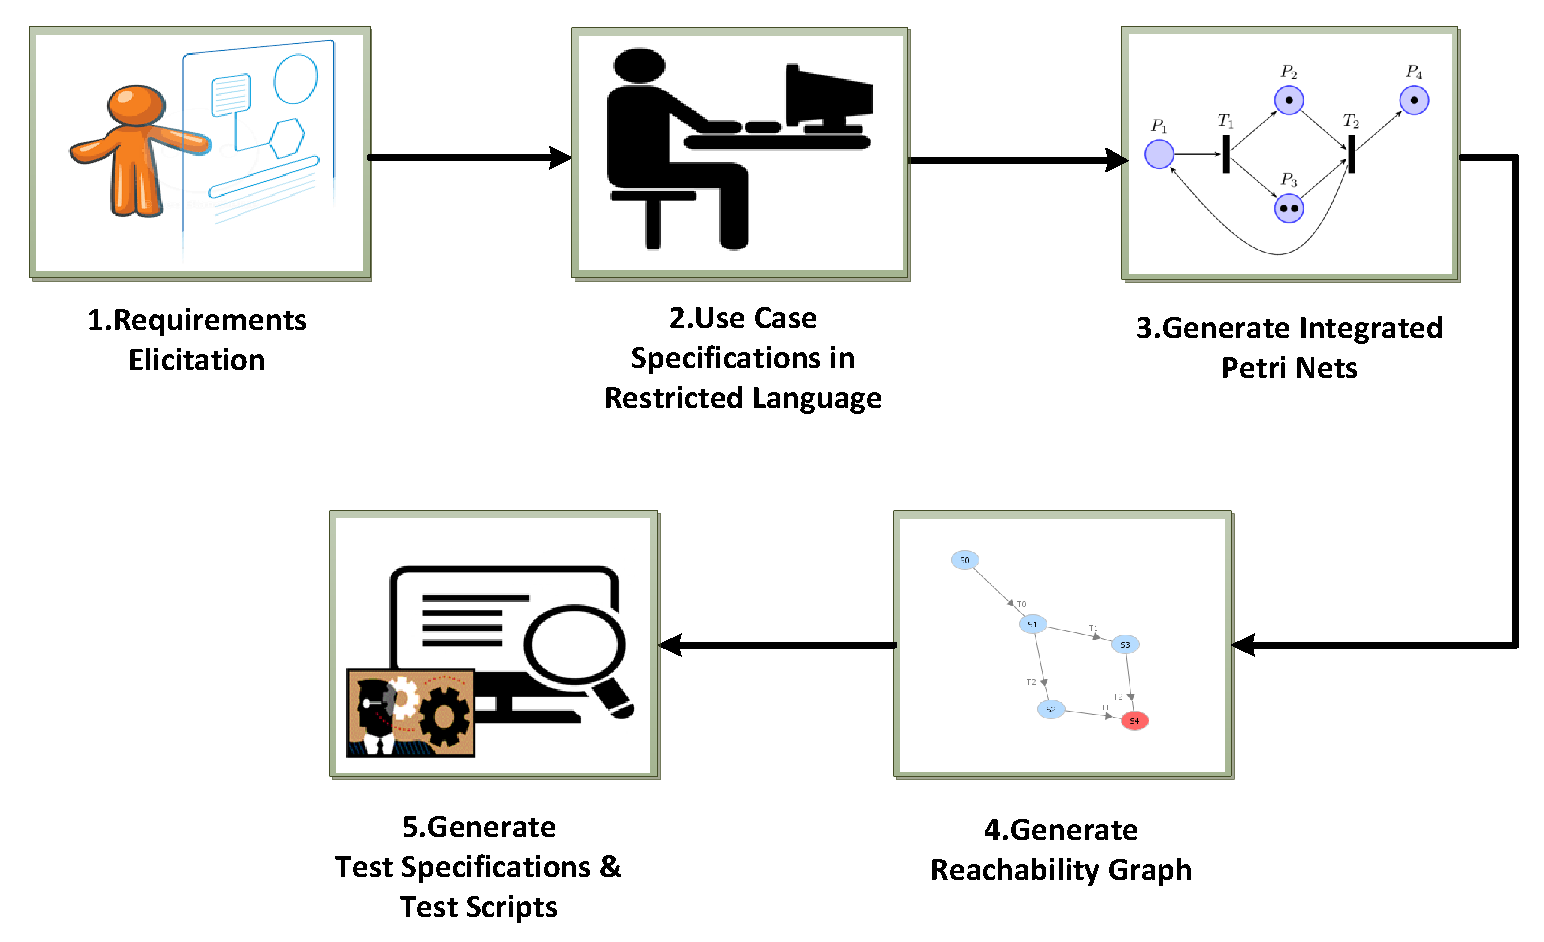
\includegraphics[width=0.9\textwidth]{content/images/Chapter1/proposed_solution.pdf}}
\caption{An overview of the proposed solution}
\label{fig:proposed_solution}
\end{figure}
\section{Thesis Management}
A project plan was created in order to guarantee an organized approach to this thesis work. Various milestones were created to monitor the progress of the project with time.
\subsection{Project Plan}
A Waterfall model with overlapping phases was created for project planning. The Gantt chart in Figure \ref{fig:gc} shows the various phases and the time duration planned for each phase. 
The significant phases are enlisted below.
\begin{enumerate}
\item Literature Survey
\item Design and Development
\item Testing and further development
\item Documentation
\end{enumerate}
From the Gantt chart, it can be seen some phases are overlapped. For example, the overall design of the approach and tool selection for implementation can be made immediately once a feasible approach has been identified in the literature survey. The identification of a suitable system and the enumeration of requirements for basic functionalities of the proposed tool can be done in parallel to the above mentioned phase.
\begin{figure}[htb!]
\centering
\fbox{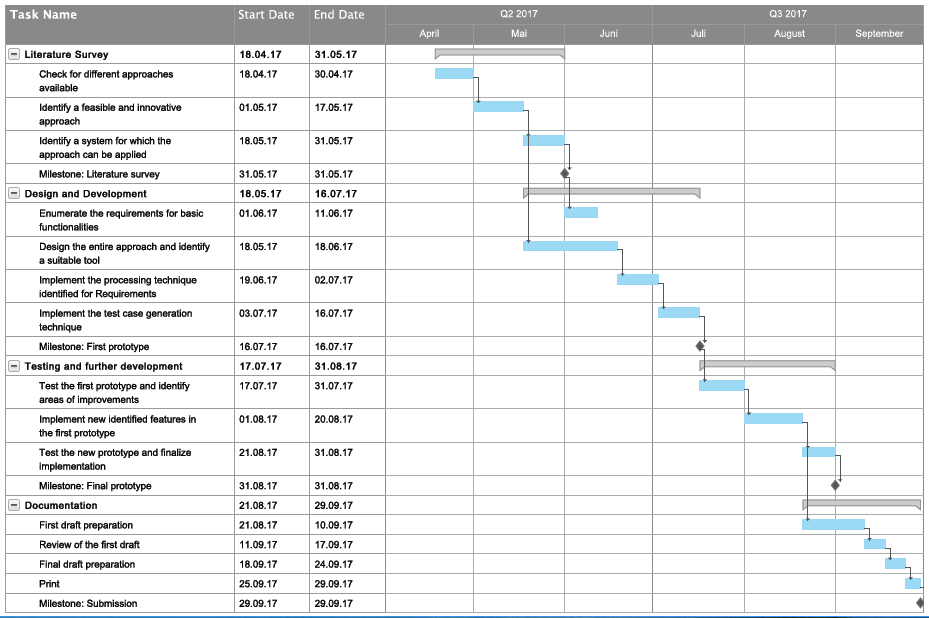
\includegraphics[scale = 0.69]{content/images/Chapter1/figure_2_ganntchart}}
\caption{Gannt Chart for the thesis work}
\label{fig:gc}
\end{figure}
\subsection{Literature Survey}
This thesis mainly revolves around the work done by Edgar et. al., 2015 \cite{sarmiento2015mapping}, Wang et. al., 2015 \cite{wang2015automatic} and Toa Yue et. al., 2015 \cite{yue2015rtcm}. The literature survey started with the books from the Library of University Stuttgart and moved towards online resources like the IEEE Xplore catalog, the ACM digital library, the E-Books from various publishers like Springer, the search engines from Internet such as Google\footnote{https://www.google.de} and specific search engines for scientific journals like Google Scholar\footnote{https://scholar.google.de}. Apart from the scientific journals and publications, numerous other resources had been used from the internet regarding the availability of different tools, their user manuals and their documentation.
\subsection{Thesis Structure}
The thesis has been organized as the following chapters.
\paragraph{Chapter 1} This chapter gives a short introduction to the thesis work, the motivation behind the thesis and a rough idea of the proposed solution.
\paragraph{Chapter 2} This chapter gives a short introduction to the different methodologies and terminologies that will be used throughout the rest of the thesis.
\paragraph{Chapter 3} This chapter provides an overview of related research work in the domain of automatic test case generation and it also gives a basic introduction to the technologies used in the implementation stage of the thesis.
\paragraph{Chapter 4} This chapter provides a detailed account of the proposed approach and the various methodologies used for test script generation.
\paragraph{Chapter 5} This chapter gives a deeper insight into the design of the tool and the implementation of the different methodologies introduced the previous chapter.
\paragraph{Chapter 6} This chapter illustrates the evaluation of the proposed tool and its comparison with other similar approaches.
\paragraph{Chapter 7} This chapter provides a short overview of the thesis and details the different limitations and contributions of the current work.
% !TeX spellcheck = de_DE
\chapter{Background}\label{background} 
This chapter gives a short introduction to topics regarding Agile processes and their definitions, Model Driven Architecture, Unified Modeling Language and Petri Nets. Basic knowledge in these topics helps us to appreciate the various design and implementation decisions taken in Chapter \ref{relatedwork} and \ref{proposedsolution}. This chapter also acts a guide to understand the various terminologies used throughout this work.

\section{Evolution of Agile Software Development}
Agile Software Development was introduced in the year 2001 by Agile Alliance to keep up with growing demands of the software industry. Traditional software development methods like Waterfall model couldn’t deliver the expected results on circumstances of frequent requirement changes and increased software complexity. The main reason that can be attributed to the failure of traditional development methods is the single flow of sequential development phases without any iterative phases.

For example, in Waterfall Model, the business analyst along with the client creates a set of requirements and a model of the final product. A requirement specification document is created which acts as the base document for the next development phases like Analysis, Design, Development and Testing of the product. The client is never involved during the development process and would view the product only after the final testing is completed. If the requirements of the client were not captured correctly or if the client has a changed requirement, then the entire development process has to be repeated. This kind of rework increases the cost, time and resources needed for the project and subsequently leads to its failure. (\cite{versionone}, \cite{getzephyr})

Agile Software Development, on the other hand, is built on the foundation of iterative approaches, in which product development happens incrementally and stakeholder participates in the entire \gls{sdlc} from the conception to the delivery of the product. One such methodology is \textit{Sprint} in which a larger functionality is broken into smaller pieces called \textit{User Stories} which can be delivered in a time span of just two weeks. This approach has several advantages such as the time consuming documentation is replaced with face to face communication with the stakeholders reducing the misinterpretation and hence a providing better understanding of stakeholder requirements.

Agile also provides separate methodologies for testing which makes testing easier with a quick feedback from stakeholders. A user story is marked complete if it passes all the acceptance tests. They are then evaluated whether to retain them for regression testing. A difference in interpretation of the requirement can be found out immediately with feedback and only a small rework will be needed in case of a difference. Test team members create the test plan, write test specifications and test cases and manage the testing activities within a sprint. The testing activities can be classified as follows.

\subsection{Requirements-Based Testing}
In this testing methodology, the objective is to verify whether the deliverables’ design and code meets the application’s requirements. Hence the test cases, conditions and data are generally derived from the requirements specification document. The testing can be done to verify either the functional attributes or the non-functional attributes like performance, reliability or usability. \cite{tahat2001requirement}

\subsection{Model-Based Testing}
This methodology involves the generation of test cases from models describing the system requirements and behavior. Even though this methodology requires the building of models up-front in the development cycle, it has several advantages like finding inconsistencies in the requirements itself and detection of discrepancies even before the code is generated. \cite{dias2007survey}

\subsection{Code-Based Testing}
In this methodology, test cases are used to evaluate the code to verify whether different test paths of the system are covered. The benefits of this methodology are that the parts of the software not tested in other techniques are covered. \cite{prasanna2005survey}

The main objective of this thesis is to simplify the existing test management process. As bulk of the effort is spent on elicitation and generation of test cases, this thesis aims to simplify the task of test case generation by using an automated tool. Most of the existing approaches for automated generation of test cases can be put under the above three categories. This thesis tries to automate test case generation for the first category which is Requirements-Based Testing.


\section{Model Driven Software Engineering}
An important paradigm shift happened in the field of software development after the introduction of \gls{mda} by \gls{omg}.   The underlying idea of \gls{mda} is to make use of models, a key tool in engineering, for software development. In general, models can be defined as abstraction of the system and its environment. An advantage with models is that it can be used to provide different levels of abstraction, with each level highlighting specific aspects or features of the system. Hence a model is essentially a representation of the necessary characteristics of the underlying system, leaving out the rest and thus contains less complexity. Less complexity of the models provides an easy way of system behavior prediction, examination of specific properties and unambiguous communication among software developers.

One of the motivations for \gls{mda} approach is that the developed software will be deployed to one or more platforms. The volatility of the platforms is higher than the higher-level models of the system and the objective of \gls{mda} is to create models that are increasingly independent of the target platform. In \gls{mda}, \glspl{pim} are initially designed in a platform independent language (e.g. \gls{uml}), which are then translated into \glspl{psm} by mapping them to some implementation language (e.g. C++, Java) as illustrated in Figure \ref{fig:Overview_MDA}.

\begin{figure}[htb!]
\centering
\fbox{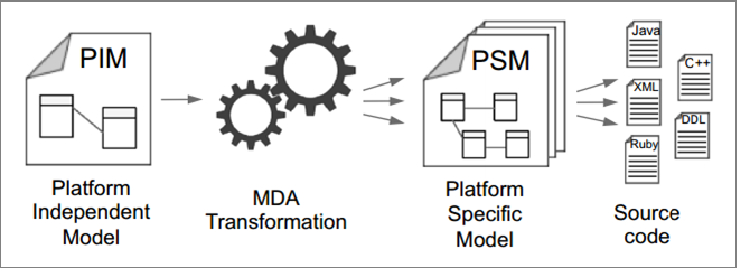
\includegraphics[width=0.8\textwidth]{content/images/Chapter2/Overview_MDA.pdf}}
\caption{Overview of transformations in MDA \cite{cerny2015separation}}
\label{fig:Overview_MDA}
\end{figure}

A number of \gls{omg} standards such as The \gls{uml}, \gls{xmi}, \gls{cwm}, \gls{mof} form the core of \gls{mda} concepts. Among these standards, \gls{uml} is used to define the \gls{pim} models which will be discussed in detail in the Section \ref{secuml} whereas the other standards are not in the scope of this thesis.

The term \gls{mdsd} or \gls{mdd} describes the family of engineering approaches that use models and their transformations for creating software products. \gls{mdsd} takes advantage of the \gls{mda} facilities, as a result of which the code can either be automatically or semi-automatically generated from models that are described in standard specification languages. The main priority of \gls{mdsd} is to enable the validation of software by the end users and customer stakeholders as early as possible in \gls{sdlc}.



\section{Unified Modeling Language} \label{secuml}
\gls{uml} is a standard from \gls{omg} and is a de-facto industry standard for modeling business applications in \gls{mdsd} \cite{cerny2015separation}. \gls{uml} models help to understand the requirements of the system graphically. They also provide aides to design the system, its components and to model the relationship existing between them right from early stages of software development. \gls{uml} also helps the developers and end users to maintain consistency in their interpretation of the design specification. \gls{uml}’s rapid gain in popularity in object oriented software development has attracted a great deal of research on \gls{uml} in software testing. (\cite{nebut2003requirements},\cite{badri2003use},\cite{nebut2003requirements})

\gls{uml} can be classified broadly into two categories namely structural and behavioral models. The structural diagrams represent the static structure of the system and the relationship between them. The different structural diagrams represent different abstraction and implementation levels. On the other hand, behavioral diagrams represent the dynamic behavior of the objects in the system i.e. the changes that happen in the system over time. Some of the important \gls{uml} diagrams which are used in upcoming sections are elaborated below.

Class Diagram is one example of structural diagrams that acts as a blueprint of the system or subsystem under development. It is extensively used to model the objects that make up the system, the relationship between them, their description and the functions they provide. Class Diagrams usage is across different levels in the development cycle. In analysis stage, it is used to understand the requirements of the problem domain whereas, in the implementation stage, it can be used to create actual software classes. An example of Class Diagram is shown in Figure \ref{fig:umldiagrams_subfigA}.

Activity Diagram is one example of behavioral diagrams which illustrates the sequence of actions in a process. Activity Diagrams usage across different levels in the development cycle are illustrated below. In requirements stage, it can be used to model the flow of events that the use cases describe and in design and implementation stage, it can be used to define the behavior of operations. An example of Activity Diagram is shown in Figure \ref{fig:umldiagrams_subfigB}.

\begin{figure}[htb!]
  \centering
    \subfloat[A UML Class Diagram]{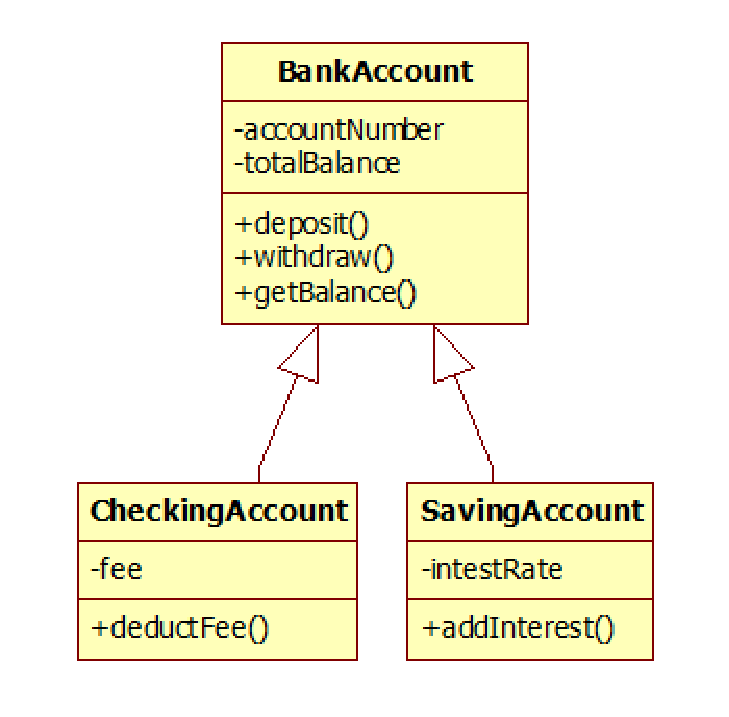
\includegraphics[width=0.45\textwidth,frame]{content/images/Chapter2/ClassDiagram.pdf} \label{fig:umldiagrams_subfigA}}
   \subfloat[A UML Activity Diagram]{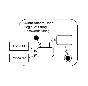
\includegraphics[width=0.45\textwidth,frame]{content/images/Chapter2/ActivityDiagram.pdf} \label{fig:umldiagrams_subfigB}}
	\caption{Examples of UML diagrams.}
\label{fig:umldiagrams}
\end{figure}

\section{Petri Net}
Petri Net is a graphical and mathematical modeling tool with well defined semantics suitable for formal analysis. The concept of Petri Net was first introduced by Carl Adam Petri in the year 1961, after which it had grown tremendously to support different domains like workflow management, manufacturing, real time systems, distributed systems, embedded systems, protocols and networks, performance evaluation and much more.
 
In the domain of computer science engineering, Petri nets are mainly used in information processing systems that can be categorized as parallel, concurrent, distributed, asynchronous, non-deterministic and stochastic. Petri nets can be used as communication documents like flow charts, block diagrams and networks but can also simulate the dynamic and concurrent activities of the system with the concept of tokens. Also, it can model the mathematical representations of the systems using algebraic and state equations. 

\subsection{Basics of Petri Net}
There are different kinds of Petri Nets depending upon the amount of information that the nets can carry. One such example of low level Petri Net is the Place/Transition Net (PT-Net) which is used in this thesis.

A Petri Net is an example of directed, bipartite and weighted graph in between two nodes called places and transitions. Arcs run between places and transitions and each place can hold specific items called tokens. An example Petri Net is shown in Figure \ref{fig:petrinet_example} and the various elements are elaborated below.

\begin{figure}[htb!]
\centering
\fbox{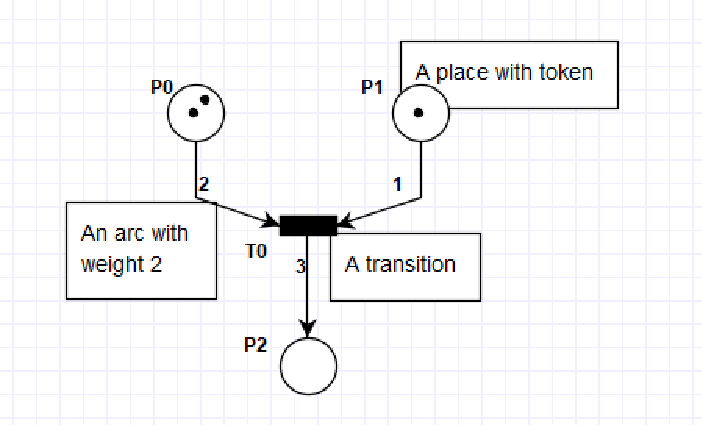
\includegraphics[width=0.6\textwidth]{content/images/Chapter2/Petrinetwithlabels.pdf}}
\caption{An example of Petri Net}
\label{fig:petrinet_example}
\end{figure}

\textbf{\textit{Places}} are the passive component of the net, and they represent the buffer, communication medium or in general a geographical location. The current state of the system is determined by the number of tokens present in a place and this state is represented by the term \textit{Marking} in Petri Nets.

\textbf{\textit{Transitions}} are the active components of the net, which represent the activities that change the state of the system. Transitions are fired only when certain preconditions are met and these conditions are represented in the net by means of tokens.

\textbf{\textit{Tokens}} are present inside the places and each token represents a condition to be fulfilled or a synchronization condition. In general, tokens represent a physical or information object.

\textbf{\textit{Arcs}} run only between places and transitions or vice versa. In the first case, these are called \textit{input arcs} whereas in the second case these are called \textit{output arcs}. Each arc is also associated with a specific weight that determines the number of tokens required for firing the particular transition.

\subsection{Formal Definition and Basic Terminology}
The terms defined in the above section can be formally defined as the following. The definitions are an excerpt from Calisaya et. al., 2015 \cite{calisaya2016analysis}.

\begin{definition}
\label{def:def1}
A \textbf{place-transition Petri Net} \cite{reisig2012petri}  is a five-tuple PN = (P, T, F, W, M$_{0}$) where P = $ \lbrace $p$_{1}$, p$_{2}$, ..., p$_{n} \rbrace $ is a finite set of places, T = $ \lbrace $t$_{1}$, t$_{2}$,..., t$_{n} \rbrace $ is a set of transitions, F   (P $\times$ T) $ \cup $ (T $\times$ P) is a set of arcs, W : F $ \subseteq $ $ \rightarrow$ $ \lbrace $1, 2,...$ \rbrace $ is a weight function, M$_{0}$ : P  $ \rightarrow\lbrace $0, 1, 2, ...$ \rbrace $ is the initial marking and P $ \cap $ T = $\emptyset $ and P $ \cup $ T 
$ \neq $ $ \emptyset $.
\end{definition}

\begin{definition}
\label{def:def2}
For a PN = (P, T, F, W, M$_{0}$), a \textbf{marking} is a function M: P $  \rightarrow$ $ \lbrace $0, 1, 2,...$ \rbrace $, where M (p) is the number of tokens in p. M$_{0}$ represents the initial marking of PN.
\end{definition}


\begin{definition}
\label{def:def3}
A \textbf{transition} t is enabled for firing at a marking M if M (p) $ \geq $ W (p, t) for any p $ \in $ p$ _{in} $ where p$ _{in} $ is the set of input places of t. On firing t, M is changed to M' such that $ \forall $p $ \in $ P: M' (p) = M (p) - W (p,t) + W (t,p). 
\end{definition}

\begin{definition}
\label{def:def4}
For a PN, a sequence of transitions $ \sigma $ = $ \langle $t$_{1}$, t$_{2}$, ..., t$_{n} \rangle $ is called a \textbf{firing sequence} if and only if M$_{0}$[t$_{1} \rangle $, [t$_{2} \rangle $,..., [t$_{n} \rangle $M$_{n}$. In notation, M$_{0}$ [PN, $ \sigma \rangle $M$_{n}$ or M$_{0}$ [$ \sigma \rangle $M$_{n}$.
\end{definition}

\begin{definition}
\label{def:def5}
For a PN = (P, T, F, W, M$_{0}$), a marking M is said to be \textbf{reachable} if and only if there exist a firing sequence $ \sigma $ such that M$_{0}$ [$ \sigma \rangle $M.
\end{definition}


\subsection{Analysis of Petri Nets}
One of the main features of Petri Net is the ability to perform analysis on model properties i.e. it can detect defects related to structural and dynamic properties \cite{murata1989petri}. A simple transversal of the flow relation between places and transitions can detect the structural properties whereas initial markings and final markings after transitions can detect the dynamic properties. As defined in \cite{reisig2012petri}, the defects due to dynamic properties of boundedness, liveliness, deadlock free and reachability can be detected using methods like simulation, reachability/coverability or invariant analysis.

 The transition behavior in a Petri Net is shown in Figure \ref{fig:petridiagrams}. Figure \ref{fig:petridiagrams} (a \& b) show Petri Nets with markings M0 and M1 respectively.  P0 and P1 are the places and T0 is the transition. The places contain tokens and arcs with arc weight of two and one respectively. This marking, which is the required precondition, enables the firing of the transition T0 and subsequently results in the marking as shown in Figure  \ref{fig:petrinet_subfigB}.  The final marking consists of place P2 with three tokens since the arc from T0 to P2 is of weight 3. 

\begin{figure}[htb!]
  \centering
    \subfloat[before transition]{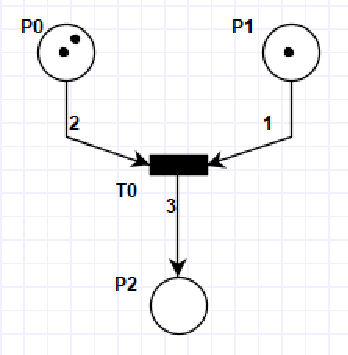
\includegraphics[width=0.4\textwidth,frame]{content/images/Chapter2/Petrineta.pdf} \label{fig:petrinet_subfigA}}
   \subfloat[after transition]{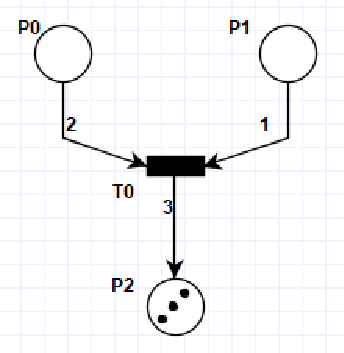
\includegraphics[width=0.4\textwidth,frame]{content/images/Chapter2/Petrinetb.pdf} \label{fig:petrinet_subfigB}}
	\caption{Concept of transitions in a Petri Net.}
\label{fig:petridiagrams}
\end{figure}



% !TeX spellcheck = de_DE

\chapter{Related Work and Utilized Software Tools}\label{relatedwork} 
The foundation for every research work is provided by other related research work in the same domain. The first section of this chapter provides an overview of such related research works for test case generation. The second half of this chapter focuses on some of the technologies used for implementing the proposed approach.

\section{Related Work}
This section provides an overview of already existing research and approaches in the domain of automatic test case generation. It also describes the way in which the proposed approach differs from the already existing approaches and how the disadvantages in the already existing approaches are eliminated. These related research works are grouped according to the type of inputs needed for test case generation. 
 
\subsection{Model Based Testing}
The following section describes the related research for automatic test case generation using a formal model of the requirements as an input artifact. Most of these approaches use \gls{uml} diagrams as a formal model.

Shirole et. al. \cite{shirole2013uml} gives an overview of different existing methodologies for test case generation from \gls{uml} models. Most of these approaches need the requirements to be converted into \gls{uml} behavioral models like state-charts (\cite{ryser1999scenario}, \cite{bandyopadhyay2009test}), sequence diagrams (\cite{nebut2003requirements}, \cite{linzhang2004generating}, \cite{briand2002uml}) and activity diagrams (\cite{nebut2006automatic}, \cite{nayak2012synthesis}).  Some of these approaches are elaborated below.

Badri et. al. \cite{badri2003use} proposes a technique of generating test cases from use cases and collaboration diagrams. The requirements are first manually converted to a use case model from which the corresponding collaboration diagrams are created. Collaboration diagrams are defined using a formal language called Collaboration Description Language, which provides a textual representation for the diagrams and subsequently test cases are generated from them.

The authors Nebut et. al. \cite{nebut2003requirements} takes use case diagrams and sequence diagrams as an input artifact to generate test cases. In order to create test cases along with test input data, the use cases are modeled with formalized expression. Here in this technique, the pre and post conditions and other relationships are defined with the help of logical expressions. Finally for test case generation, the use case parameters are initialized with inputs and the logical expressions are solved to derive the test cases and along with the corresponding inputs.

Tahat et. al. \cite{tahat2001requirement} proposed a technique to generate test cases from requirements defined in \gls{sdl} (\cite{algayres2012goal}, \cite{bochmann1997automating}, \cite{bromstrup1995tesdl}). Initially, each requirement is first converted into a \gls{sdl} system model and then a combined \gls{sdl} model for the entire set of requirements is created manually. This combined model is converted into \gls{efsm}. This acts as an input artifact for the test case generation process.

The drawbacks of the above approaches are as follows. The creation of formal models is common only in case of object oriented applications and there are domains like embedded systems where models are not so common. In such scenarios, creation of formal models is an overhead and an approach that could evade this is greatly appreciated. Even in industries that have embraced \gls{mda} approach, the creation of precise behavior models is expensive and hence it is not a frequently used practice.

Our work differs from all the above mentioned methodologies in that it does not need a formal model either for test creation or for obtaining test data and is completely automated that it does not require any manual intervention in any stage of test case generation.

\subsection{Natural Language Processing Based}
Different approaches that generate test case using \gls{nlp} techniques are present but mostly these methods require additional behavioral model inputs like state diagrams \cite{ryser1999scenario}, activity diagrams \cite{hasling2008model}, labeled transition diagram \cite{katara2006making} or they need provision of additional inputs such as test data or manual test derivation \cite{bertolino2003use}. There are also several other approaches existing (\cite{frohlich2000automated}, \cite{yue2010automated}, \cite{yue2013facilitating}) for generating \gls{uml} models from \gls{nl} requirements. They can also be easily adapted for test case generation.

The approach proposed by Kulkarni and Joglekar \cite{kulkarni2014generating} makes use of \gls{nlp} tools to parse the requirements written in natural language and convert them into graph-based structures called Knowledge Representation. This graph is then analyzed to create test cases. The objective of authors Ryser et. al. \cite{ryser1999practical} is to create system test cases from scenarios expressed in \gls{nl}. But since scenarios described in natural language tend to be more ambiguous, an intermediate formal representation is created. State Machines are used as a formal representation, which are then used for test case generation.

Barros et. al. \cite{barros2011ucscnl} makes use of use case specifications to generate test cases. But the language used to define the specifications is controlled i.e. only part of natural language grammar and structure can be used. In this work, this controlled language is called ucsCNL and test cases are automatically generated from use case specifications.

Our model makes use of \gls{nl} requirements as inputs but does not require the formal intermediate \gls{uml} models and presence of domain experts to verify these models. Instead it is a completely automatic process where a \gls{nl} requirement input results in corresponding executable test scripts.  

\subsection{Keyword Driven Testing}
\gls{kdt}, also called Table Driven Testing or Action Word Testing, is a testing methodology which defines keywords to describe operations and actions. It is greatly suited for test automation and there exists a variety of approaches that can generate executable test scripts. Even though the following literatures have not directly contributed for the test case generation in our work, they were of immense help in defining a test script generation methodology.

Tang et. al. \cite{tang2008towards} has proposed a methodology in which test cases can be derived for \gls{kdt}. This technique even produces test scripts suitable for different test applications or \glspl{sut} under different environments. Keywords identify the atomic operations in test execution and are very much dependent on their application. For example, \textit{Click} and \textit{Connect} are the keywords for GUI and Database Applications respectively. Test cases are created by the users by specifying a sequence of keywords i.e. the actions and these test cases are then converted into test scripts which act as an input to the test driver specific to an environment.

Little and Miller \cite{little2006translating} proposed a similar approach where keyword commands are converted to executable test scripts. Hametner et. al. \cite{hametner2012agile} suggested a test case generation technique for \gls{kdt} in the field of industrial automation systems. Here, test engineers write test cases manually using predefined keywords and a predefined tabular template in a high abstraction level. The automated generation of test cases is not supported in this technique but can be easily adapted. Thummalapenta et. al. \cite{thummalapenta2012automating} put forth a technique in which test scripts can be created from manually written test cases which consists sequences of tuples like \textit{action-target-data}.


\subsection{UMTG – A hybrid approach}
This section describes an approach which is a hybrid between different approaches seen above. Wang et. al., 2015 \cite{wang2015automatic} describes a semi-automatic approach for generating test cases. The approach is labeled as \gls{umtg}. The requirements are specified in a restricted natural language in a defined template called \gls{rucm} \cite{yue2015rtcm}. They are used as one of the inputs whereas the other input is the domain model of the system which has to be manually developed. This approach also needs the restrictions of the model to be modeled manually as \gls{ocl} constraints. 

\section{Utilized Software Tools}

\subsection{UMTG – A hybrid approach}
This section describes an approach which is a hybrid between different approaches seen above. Wang et. al., 2015 \cite{wang2015automatic} describes a semi-automatic approach for generating test cases. The approach is labeled as \gls{umtg}. The requirements are specified in a restricted natural language in a defined template called \gls{rucm} \cite{yue2015rtcm}. They are used as one of the inputs whereas the other input is the domain model of the system which has to be manually developed. This approach also needs the restrictions of the model to be modeled manually as \gls{ocl} constraints.

% !TeX spellcheck = de_DE
\chapter{The Proposed Solution}
This chapter gives a detailed explanation of the proposed approach and the various steps involved in it. It elaborates on the theoretical design behind the conversion of agile requirements described in natural language into formal models and the subsequent test case generation methodologies.
 
The first section of this chapter gives an overview of the proposed solution and the different steps involved in it. The following sections elaborate the steps defined in the overview and the justification on which the theoretical ideas are chosen.


\section{Overview of the solution}
The proposed solution of test script generation from requirements can be broadly classified into four important steps.
\begin{enumerate}
\item Requirements in a Restricted Natural Language.
\item Generation of Petri-Nets from Use Case Specifications.
\item Generation of Reachability/Coverability Graph.
\item Generation of Test Specifications and Test Scripts.
\end{enumerate}
Figure \ref{fig:proposed_solution2} shows the skeleton of the proposed work. The detailed explanation for these steps can be found in the following sections.

\begin{figure}[]
\centering
\fbox{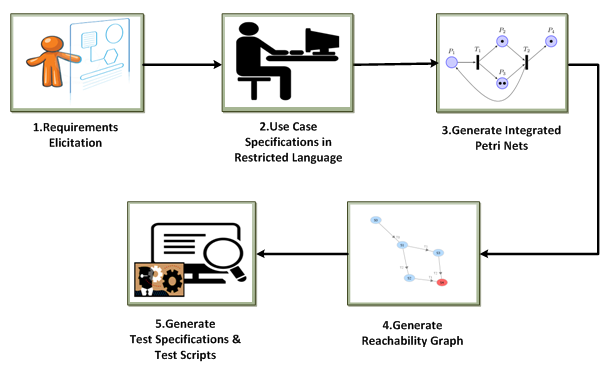
\includegraphics[width=0.9\textwidth]{content/images/Chapter4/proposed_solution.png}}
\caption{An overview of the proposed solution}
\label{fig:proposed_solution2}
\end{figure}


\section{Requirements in a Restricted Natural Language}
The main objective of this approach is to generate test cases directly from requirements specified in natural language. In the industry, one of the important documents used to communicate requirements between the different stakeholders is \glspl{ucs}. In order to reduce the incompleteness and imprecision in \glspl{ucs}, a template with restriction rules are usually used, thereby making it a semi-formal representation. 

\subsection{RUCM – A Restricted Natural Language}
\gls{rucm} \cite{yue2013facilitating} is one such use case format that provides restriction rules and specific keywords, hence confining the use of natural language for \glspl{ucs}. It also corresponds to a specific metamodel called UCMeta, which facilitates automatic analysis of use cases. The selection of a restricted \gls{nl} template depends upon factors like simplicity, expressive power, better understandability and quality of models derived from it. Experiment results \cite{yue2013facilitating} shows that the template is beneficial and is applicable in various scenarios with the above mentioned characteristics.

\subsection{Restriction Rules and Keywords}
\gls{rucm} has also defined a list of standard keywords. A short overview of the rules is given below. For example, a conditional logic sentence is defined by the keyword IF-THEN-ELSEIF-ELSE-ENDIF, a concurrency statement by keyword MEANWHILE, condition checking sentences by keyword VALIDATES THAT and iteration sentences by DO-UNTIL. RESUME STEP keyword is used when the alternative flow should return back to its reference flow. Similarly ABORT keyword is used to describe an exit action due to some exceptions.  The complete set of keywords can be found in the template reference given in \cite{yue2013facilitating}. In addition to the keywords, \gls{rucm} also specifies restriction rules that are detailed in \cite{yue2013facilitating}. A table describing the basic elements of a \gls{rucm} template is given in Table \ref{tab:rucmtemplate}.

% Table generated by Excel2LaTeX from sheet 'Sheet1'
\begin{table}[htbp]
  \centering
  \caption{RUCM Use Case Template}
	\begin{adjustbox}{width=1\textwidth}
    \begin{tabular}{|l|l|l|l|l|l|l|l|}
    \toprule
    Element & \multicolumn{7}{l|}{ Description} \\
    \midrule
    Use Case Name & \multicolumn{7}{l|}{ The name of the use case. It usually starts with a verb.} \\
    \midrule
    Brief Description  & \multicolumn{7}{l|}{Summarizes the use case in a short paragraph.} \\
    \midrule
    Precondition & \multicolumn{7}{l|}{ What should be true before the use case is executed.} \\
    \midrule
    Primary Actor  & \multicolumn{7}{l|}{The actor which initiates the use case.} \\
    \midrule
    Secondary Actors & \multicolumn{7}{l|}{ Other actors the system relies on to accomplish the services of the use case.} \\
    \midrule
    Dependency & \multicolumn{7}{l|}{ Include and extend relationships to other use cases.} \\
    \midrule
    Generalization & \multicolumn{7}{l|}{ Generalization relationships to other use cases.} \\
    \midrule
    \multirow{3}[6]{*}{Basic Flow} & \multicolumn{7}{l|}{ Specifies the main successful path, also called “happy path.”} \\
\cmidrule{2-8}          & \textbf{Steps (numbered) } & \multicolumn{6}{l|}{Flow of events.} \\
\cmidrule{2-8}          & \textbf{Postcondition} & \multicolumn{6}{l|}{ What should be true after the basic flow executes.} \\
    \midrule
    \multicolumn{1}{|l|}{\multirow{4}[8]{*}{Specific \newline{}Alternative Flows}} & \multicolumn{7}{l|}{Applies to one specific step of the basic flow.} \\
\cmidrule{2-8}          & \textbf{RFS} & \multicolumn{6}{l|}{ A reference flow step number where flow branches from.} \\
\cmidrule{2-8}          & \textbf{Steps (numbered)} & \multicolumn{6}{l|}{ Flow of events.} \\
\cmidrule{2-8}          & \textbf{Postcondition} & \multicolumn{6}{l|}{ What should be true after the alternative flow executes.} \\
    \midrule
    \multicolumn{1}{|l|}{\multirow{3}[6]{*}{Global Alternative\newline{} Flows}} & \multicolumn{7}{l|}{ Applies to all the steps of the basic flow.} \\
\cmidrule{2-8}          & \textbf{Steps (numbered)} & \multicolumn{6}{l|}{ Flow of events.} \\
\cmidrule{2-8}          & \textbf{Postcondition} & \multicolumn{6}{l|}{ What should be true after the alternative flow executes.} \\
    \midrule
    \multicolumn{1}{|l|}{\multirow{4}[8]{*}{Bounded \newline{}Alternative Flows}} & \multicolumn{7}{l|}{Applies to more than one step of the basic flow, but not all of them.} \\
\cmidrule{2-8}          & \textbf{RFS} & \multicolumn{6}{l|}{ A list of reference flow steps where flow branches from.} \\
\cmidrule{2-8}          & \textbf{Steps (numbered)} & \multicolumn{6}{l|}{ Flow of events.} \\
\cmidrule{2-8}          & \textbf{Postcondition} & \multicolumn{6}{l|}{ What should be true after the alternative flow executes.} \\
    \bottomrule
    \end{tabular}%
	\end{adjustbox}
  \label{tab:rucmtemplate}%
\end{table}%


\gls{rucm} was basically created for analysis of use cases and not for test case generation. Hence few additional restrictions were added to \gls{rucm} by the authors of \cite{wang2015umtg}. In order to establish composite conditions with multiple specific alternative flows, the authors decided that the specific alternative flow should also begin with the keyword IF....THEN.  Further additions to the restriction rules can be found in \cite{wang2015umtg}. This work has also made some assumptions and changes to the \gls{rucm} template which will be detailed in Chapter \ref{implementation}.
 
\subsection{Comparison with a related RNL}
Another widely used Restricted Natural Language Specification is the Scenario Specifications. It also uses restricted vocabulary and introduces restriction rules similar to \gls{rucm}. According to the author in \cite{calisaya2016analysis}, a scenario is a collection of partially ordered event occurrences, each guarded by a set of conditions (pre or post) or restricted by constraints. Further details on the scenario specifications can be found in the literature (\cite{do2000scenario}, \cite{calisaya2016analysis}).

An initial comparison between the two templates revealed the following conclusions. Scenario Specification is deprived of certain properties like the metamodel defined is not exhaustive and hence it cannot be used for complete test case generation. \gls{rucm} is more suited for safety critical embedded software and an industrial case study with this template yielded good results \cite{wang2015umtg}. Test data generation is easier with the help of \gls{rucm} since natural language processing can be introduced early in the process because of the detailed metamodel. 

Scenario Specification, on the other hand, has been used to specify requirements in natural language and subsequently to automate the check of correctness, consistency, completeness and unambiguity properties of the requirements in \cite{calisaya2016analysis}. The work in the mentioned literature also makes use of Petri Nets as a formal model for the analysis. This work uses \gls{rucm} as a template for \gls{rnl} requirement specifications and the work using Scenario Specifications as a foundation for transformation to formal models. 


\section{Generation of Petri Nets from Use Case Specifications}
One of the main objectives of this work is to establish a formal model for the requirements specified in natural language. The formal model in our work is Petri Nets, to be precise Place-Transition Petri Net, which is a sub category of Petri Nets. To establish the conversion from \gls{ucs} to PN, we use the concept of Model-to-Model (M2M) transformations. For this purpose, the \glspl{ucs} are described as a metamodel and we use \gls{rucm} as a template for this. Petri Net, on the other hand, can also be described as a metamodel.

The transformation method from \gls{ucs} to PN consists of three main steps.

\begin{enumerate}
\item The first step defines mapping rules that translate the \gls{rucm} elements into corresponding Petri Net elements according to transformation rules defined in Figure \ref{fig:rules}. The expected result of this process is a Sub Petri Net which consists of at least one place, transition and arc.
\item The second step is to compose the sub Petri Nets generated from the previous step into a whole Petri Net. This is done by the fusion of output and input dummy places between sequential sub Petri Nets or by integrating Petri Nets of other referenced \glspl{ucs}.
\item The third step is to generate an integrated Petri Net from the partial Petri Nets generated for each \gls{ucs}. According to \gls{rucm} specification, each \gls{ucs} can reference another \gls{ucs} and hence the need arises to transform referenced \gls{ucs} into a Petri Net. This step integrates the partial Petri Nets into an Integrated Petri Net and hence it reflects the properties of the synthesized partial Petri Nets.
\end{enumerate}

%\begin{figure}[htb!]
%\centering
%\fbox{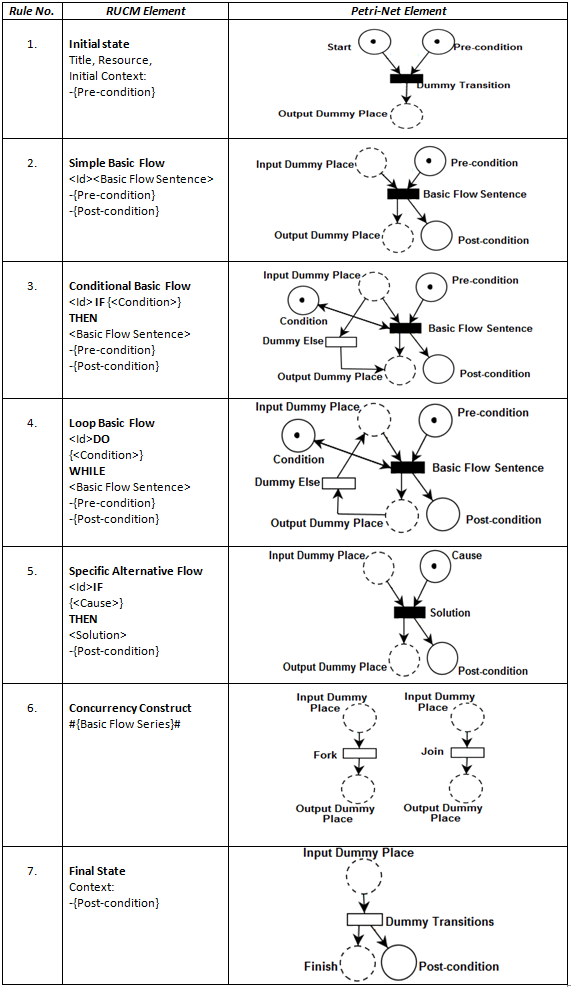
\includegraphics[width=0.8\textwidth]{content/images/Chapter4/Rules.png}}
%\caption{Model-to-Model(M2M) Transformation Rules}
%\label{fig:rules}
%\end{figure}


The different transformations and metamodels are detailed in Chapter \ref{implementation} along with a running example. As a result of the above transformations, we obtain a Petri Net that is equivalent for the given \gls{ucs}.

\begin{figure}[htb!]
  \centering
    \subfloat[first transition]{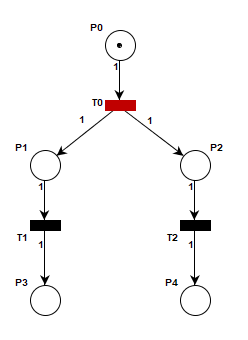
\includegraphics[width=0.3\textwidth,frame]{content/images/Chapter4/first.png} \label{fig:rg_subfigA}}
   \subfloat[second transition]{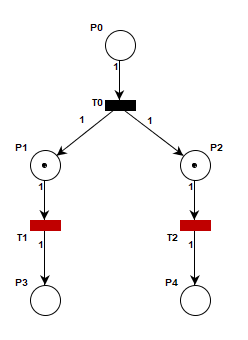
\includegraphics[width=0.3\textwidth,frame]{content/images/Chapter4/second.png} \label{fig:rg_subfigB}}
   
     \subfloat[third transition]{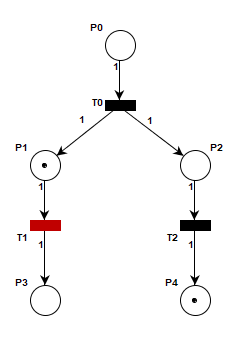
\includegraphics[width=0.3\textwidth,frame]{content/images/Chapter4/third.png} \label{fig:rg_subfigC}}
   \subfloat[fourth transition]{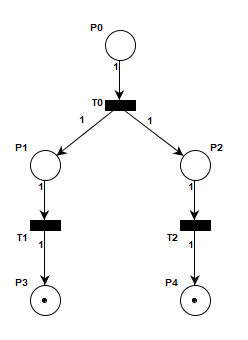
\includegraphics[width=0.3\textwidth,frame]{content/images/Chapter4/fourth.png} \label{fig:rg_subfigD}}
	\caption{Concept of Reachability.}
\label{fig:rgconcept}
\end{figure}

\section{Generation of Reachability/Coverability Graph}
As mentioned in Chapter \ref{background}, one of the important properties of Petri Net for dynamic analysis is reachability. As already described, when a transition is enabled for firing, tokens are transferred between places. This causes a change in marking of the Petri Net and each marking is defined by the term \textit{state}. Thus a new state is reached from the initial state. A \textit{reachable state} is defined as a state that can be reached from the current state (marking).

The Figure \ref{fig:rgconcept} explains the above process with the help of Petri Nets. The firing sequence of transitions described in the figure is $ \lbrace $T0, T2, T1$ \rbrace $. Initial marking of the Petri Net is given by $ \lbrace $1, 0, 0, 0, 0$ \rbrace $ which corresponds to $ \lbrace $P0, P1, P2, P3, P4$ \rbrace $. After the first firing, the marking of the Petri Net changes to $ \lbrace $0, 1, 1, 0, 0$ \rbrace $. As defined, these markings are also termed as states and in our case they are termed as S0 and S1 respectively. Hence it can be seen that S1 is a reachable state from S0.

A reachability or coverability graph is a graph that contains reachable markings or states as nodes and transitions, which cause the flow of tokens, as arcs. This graph contains all the possible reachable states from the initial state and can even have multiple paths. Reachability graph for the configuration given in Figure \ref{fig:rg_subfigA} is shown in Figure \ref{fig:rgexp}. Here, it can be seen that for the state S1 there are two possible reachable states namely S2 and S3 and hence contains two paths. The path described in Figure \ref{fig:rg_subfigC} is $ \lbrace $S0, S1, S2, S4$ \rbrace $ whereas there is an additional path $ \lbrace $S0, S1, S3, S4$ \rbrace $ in the reachability graph.

\begin{figure}[htb!]
\centering
\fbox{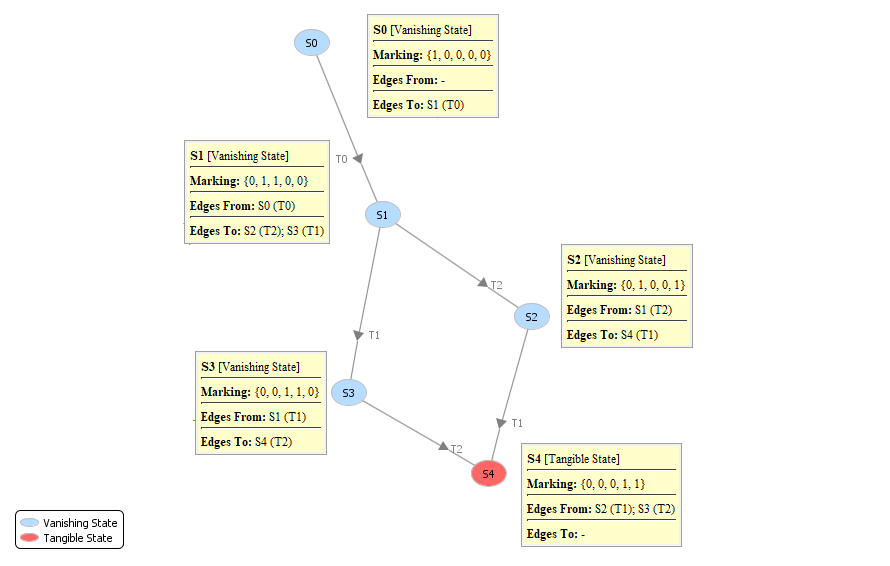
\includegraphics[scale=0.9]{content/images/Chapter4/fifth.png}}
\caption{An example of Reachability Graph}
\label{fig:rgexp}
\end{figure}

\section{Generation of Test Specifications and Test Scripts}
The Reachability Graph acts as an input for the generation of Test Specifications and Scripts. A Reachability Graph is composed of tangible and vanishing states with transitions (from Petri Nets) acting as arcs. A tangible state is a final reachable state from a given initial state whereas a vanishing state is a state that is traversed before reaching a tangible state. Now each path from initial state to a tangible state forms a test scenario since each arc represents a transition from Petri Net. A test scenario is a sequence of actions performed to reach a particular state. In order to make these test scenarios into complete test specifications, we add other elements like Pre-Conditions, Post-Conditions and conditions from logical statements, etc. 

The test specifications consist of a set of test cases and each test case in turn is made up of a set of test steps. In practice, the test scripts are realized as a set of test steps that are implemented as packages in platform specific languages. A mapping table is created to map each of the test steps to specific packages in platform specific languages. For test data, the numerical values from test steps are extracted and used for test script generation.






% !TeX spellcheck = de_DE
\chapter{Design and Implementation of the Tool} \label{implementation} 
This chapter speaks in detail about the \gls{tsgt}. It elaborates on the design and implementation details of the tool. The entire implementation is explained with the help of a runninng example.
 
The chapter can be broadly classified into two sections. The first section speaks about the various objectives that the system has to fulfill, following that the constraints regarding the design are discussed and finally the tool design. The second section explains the various implementation details and intermediate artifacts.

\section{Design of the Tool}
The following sections elaborate on the different aspects of the tool design and the different considerations made for it.
\subsection{Design Goals}
The high level objective of the tool is to automate the test script generation process using any formal method. While analyzing the requirements of the tool in detail, following salient objectives of the tool are identified.
\begin{itemize}
\item The main goal of the \gls{tsgt} is to generate test scripts for system testing from requirements defined in the natural language.
\item The tool should also provide means for extension so that test script generation for component and unit level testing can be accommodated.
\item The primary output of the tool has to be automatically generated Test Scripts that can be directly executed on a given system. The tool should also provide Test Specifications as an intermediate output.
\item The tool should be able to provide a formal model as an intermediate output. The objective is to use the formal model for other processes in \gls{sdlc}.
\item The intermediate output should be represented in a standard format so that the artifact is compatible with other tools already available in research and industry.
\item The transformation between different models should have defined rules and should be implemented using established processes. This is to ensure that the same transformation does not yield different outputs.
\item The tool must improve the coverage of the requirements than the manual process of test case generation.
\item The tool should be automated as much as possible to reduce the time taken for test script generation.
\item The tool must try to reduce the number of intermediate input artifacts which should be manually created. This ensures increased automation.
\end{itemize}


\subsection{Design Constraints}
In this section, some of the constraints that hinder the tool implementation are discussed. This section also gives an overview of the considerations made in the design to circumvent these constraints.

One of the most important constraints is that the metamodel provided for \gls{rucm} is too detailed. This increases the complexity of converting it into a formal model i.e. Petri Net. Therefore, a less complex metamodel is created which addresses some of the main required features. This metamodel can be considered as a subset of the original metamodel. Some of the rules in \gls{rucm} are also replaced with new rules according to the requirements of our current implementation. A brief overview of the changes is given in the respective sections.

\begin{figure}[htb!]
\centering
\fbox{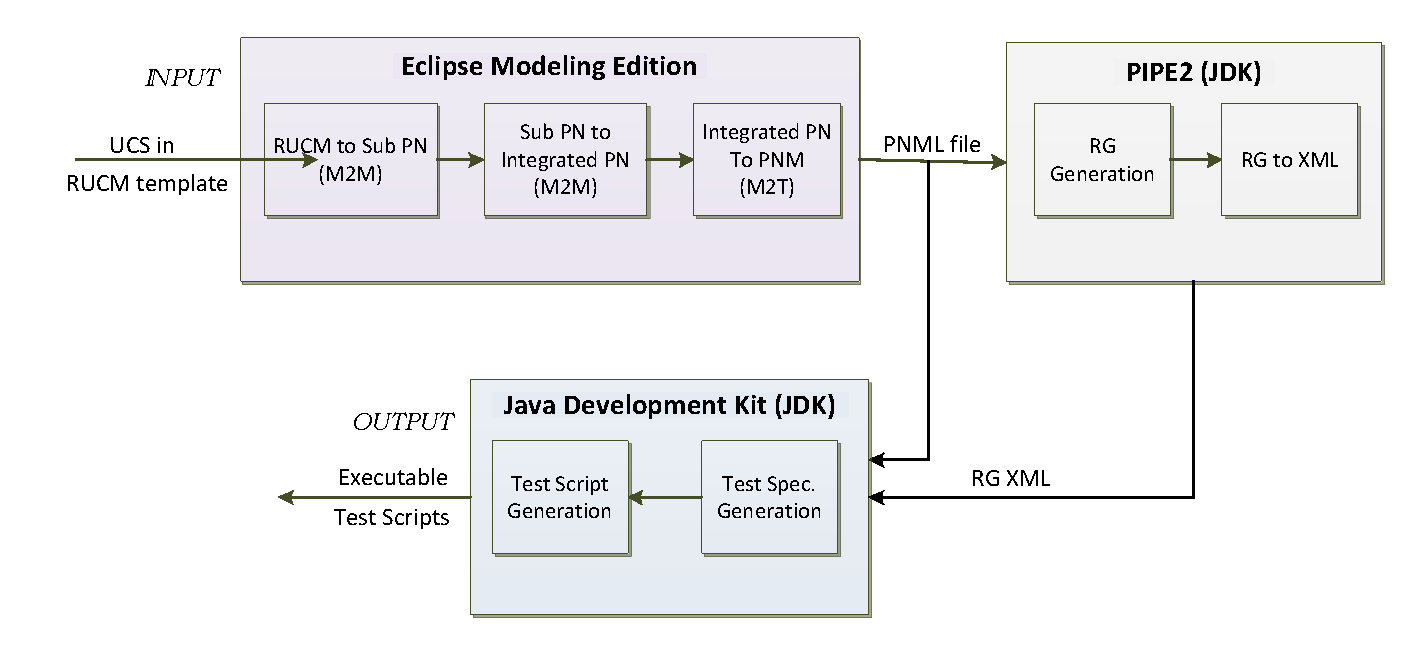
\includegraphics[width=1\textwidth]{content/images/Chapter5/SystemDesign.pdf}}
\caption{Overview of different components in the tool}
\label{fig:systemdesign}
\end{figure}

Next important constraint is the need for an intermediate input artifact that describes the environment for which the test script has to be generated. In industry, usually the test scripts are implemented using tools and a mapping is needed to interface our implementation with the specific tool implementation.  Hence for this purpose, an implementation similar to a Lookup table is used in our tool design.

\subsection{System Design of the Tool}
Figure \ref{fig:systemdesign} shows the high level system design of the tool. The design tries to incorporate the design goals described in the previous section taking into account the different limitations. The design can be divided into three blocks based on the platform on which they are implemented. The three blocks are implemented in Eclipse Modeling Edition, PIPE2 and \gls{jdk} respectively. The input of the system is \gls{ucs} in natural language and the outputs are executable test scripts. Figure \ref{fig:systemdesign} also gives the details of different sub components in each block.

\section{Implementation of the Tool}
This section describes the implementation of various blocks defined in the previous section.

\subsection{Implementation in Eclipse Modeling Edition}
\subsubsection{Metamodels Developed}
This section explains in detail about the different metamodels that are developed for the implementation of the tool. The metamodels are developed using the Eclipse Modeling Project \cite{eclipse}.
\begin{figure}[htb!]
\centering
\fbox{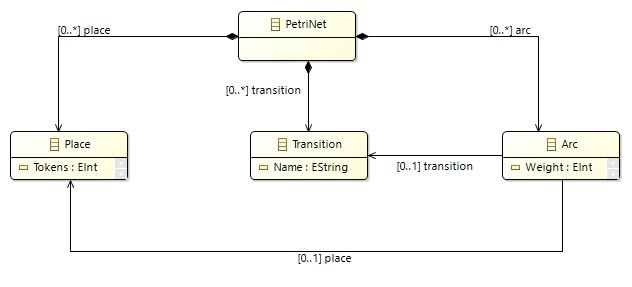
\includegraphics[width=0.7\textwidth]{content/images/Chapter5/PetriNetMetaModel}}
\caption{Petri Net Metamodel}
\label{fig:petrimetamodel}
\end{figure}

\begin{figure}[htb!]
\centering
\fbox{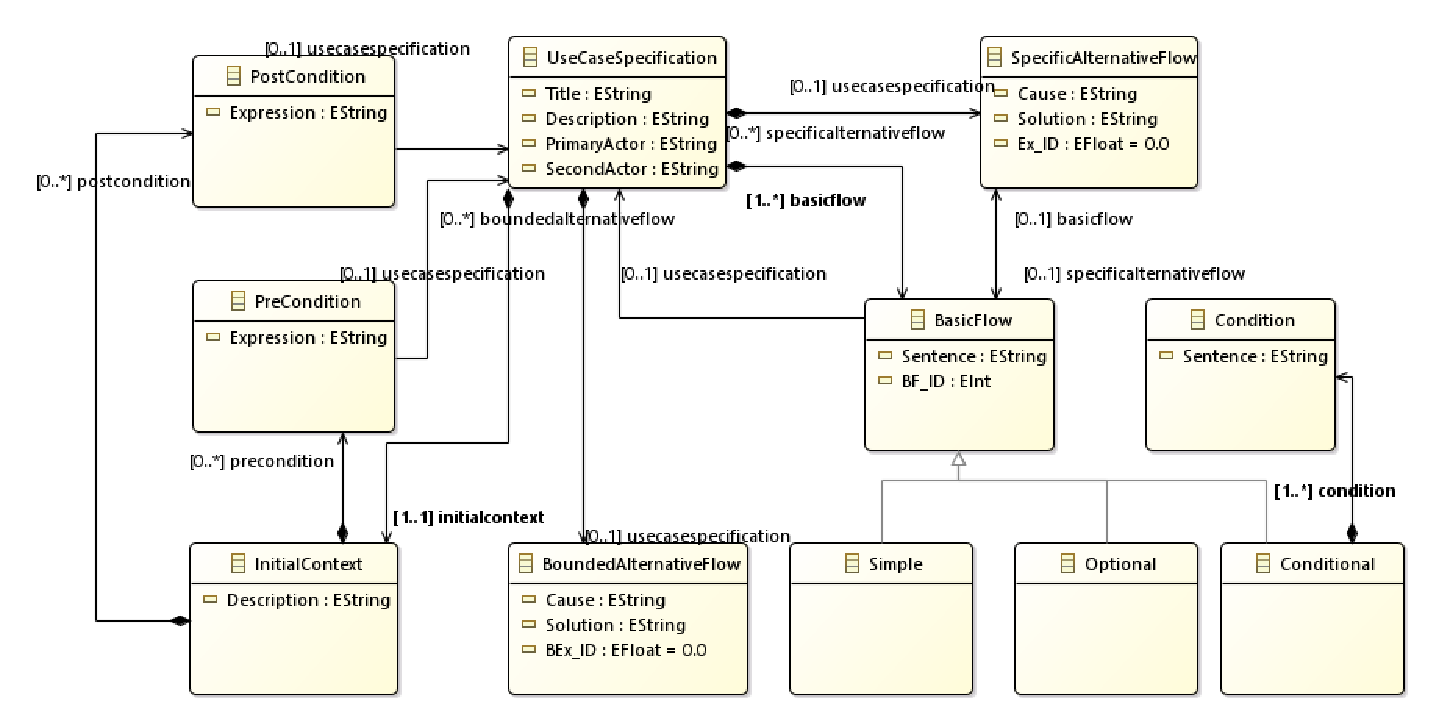
\includegraphics[width=1.05\textwidth]{content/images/Chapter5/UseCaseMetaModel}}
\caption{RUCM Metamodel}
\label{fig:rucmmetamodel}
\end{figure}

Petri Nets in our tool is based on the metamodel shown in Figure \ref{fig:petrimetamodel}. As explained earlier, it consists of Places, Transitions and Arcs. 

The second metamodel developed is for the \gls{rnl} template. The \gls{rnl} used in our case is \gls{rucm} and the metamodel for its template is shown in Figure \ref{fig:rucmmetamodel}. Here some customization according to our design goals is made. The developed metamodel is a simplified version of the metamodel in \cite{yue2013facilitating} and models only the key features necessary for our tool. It is based more on the metamodel provided in \cite{calisaya2016analysis}. Some changes are made to the restriction rules such as the rule that mandates each alternative flow should begin with a conditional statement is added and the rule that mandates the presence of post condition in each basic flow is withdrawn. 

\subsubsection{Running Example}
The tool implementation described in the next sections is explained with the help of a running example. The system under consideration is \gls{lms} from Automotive Software. The \gls{lms} is used to enhance the safety of an automobile. The purpose of the system is to help the driver to keep the vehicle in their lane to avoid crashes. 

% Table generated by Excel2LaTeX from sheet 'Sheet1'
\begin{table}[htbp]
  \centering
  \caption{Running Example}
    \begin{adjustbox}{width=1\textwidth}
    \begin{tabular}{|l|l|l|l|l|l|l|l|}
    \toprule
    \textit{\textbf{Element}} & \multicolumn{7}{l|}{\textit{\textbf{ Description}}} \\
    \midrule
    \textbf{Use Case Name} & \multicolumn{7}{l|}{\textit{Disable System}} \\
    \midrule
    \textbf{Brief Description } & \multicolumn{7}{l|}{The LMS should be turned off at certain conditions.} \\
    \midrule
    \multirow{2}[4]{*}{\textbf{Precondition}} & \multicolumn{7}{l|}{1. LMS is activated} \\
\cmidrule{2-8}          & \multicolumn{7}{l|}{2. Vehicle Speed is greater than 15 kmph} \\
    \midrule
    \textbf{Primary Actor } & \multicolumn{7}{l|}{Driver, LMS Control Unit} \\
    \midrule
    \textbf{Secondary Actors} & \multicolumn{7}{l|}{LCS, LKS and LWKS Control Units} \\
    \midrule
    \multirow{6}[12]{*}{\textbf{Basic Flow}} & \multicolumn{7}{l|}{1. The driver deaccelerates the vehicle.} \\
\cmidrule{2-8}          & \multicolumn{7}{l|}{2. The driver accelerates the vehicle.} \\
\cmidrule{2-8}          & \multicolumn{7}{l|}{3. The driver drifts away from the current lane.} \\
\cmidrule{2-8}          & \multicolumn{7}{l|}{4. The driver activates the LKS system.} \\
\cmidrule{2-8}          & \multicolumn{7}{l|}{5. The LKS steers the vehicle.} \\
\cmidrule{2-8}          & \multicolumn{7}{l|}{6. The vehicle is moving through a road under repair.} \\
    \midrule
    \multicolumn{1}{|l|}{\multirow{4}[8]{*}{\textbf{Specific \newline{} Alternative Flows}}} & \multicolumn{7}{l|}{1.1 IF Vehicle Speed less than 15 kmph THEN deactivate LMS system with an audio alert.} \\
\cmidrule{2-8}          & \multicolumn{7}{l|}{3.1 IF the departure is unintentional THEN create an audio alert and deactivate LMS system.} \\
\cmidrule{2-8}          & \multicolumn{7}{l|}{5.1 IF the driver manually takes over THEN raise an alert and deactivate LKS.} \\
\cmidrule{2-8}          & \multicolumn{7}{l|}{6.1 IF the road markers are unclear THEN raise an alert and deactivate LMS} \\
    \bottomrule
    \bottomrule
    \end{tabular}%
    \end{adjustbox}
  \label{tab:runningexample}%
\end{table}%


The \gls{lms} consists of three main components namely a \gls{lcs}, a \gls{ldws} and a \gls{lks}. The \gls{ldws} alerts the driver in case of unintentional lane changes. The \gls{lcs} and \gls{lks} will work together to take control of the vehicle and keep the vehicle in driver defined center of the lane. Table \ref{tab:runningexample} is an extract from the \gls{srs} document of \gls{lms} and it illustrates a specific Use Case called Disable System. The template used for specifying this Use Case is \gls{rucm} template and it is based on the metamodel described in the previous section.

\subsubsection{Input for \gls{tsgt}}
The next important step is to provide the input to the tool in the form of \gls{rucm} template. Once the input is entered, it should also be validated according to the template rules. For this, once the metamodels are developed, they should be exported as plug-ins and installed in the current host of Eclipse Modeling Edition.

\begin{figure}[htb!]
\centering
\fbox{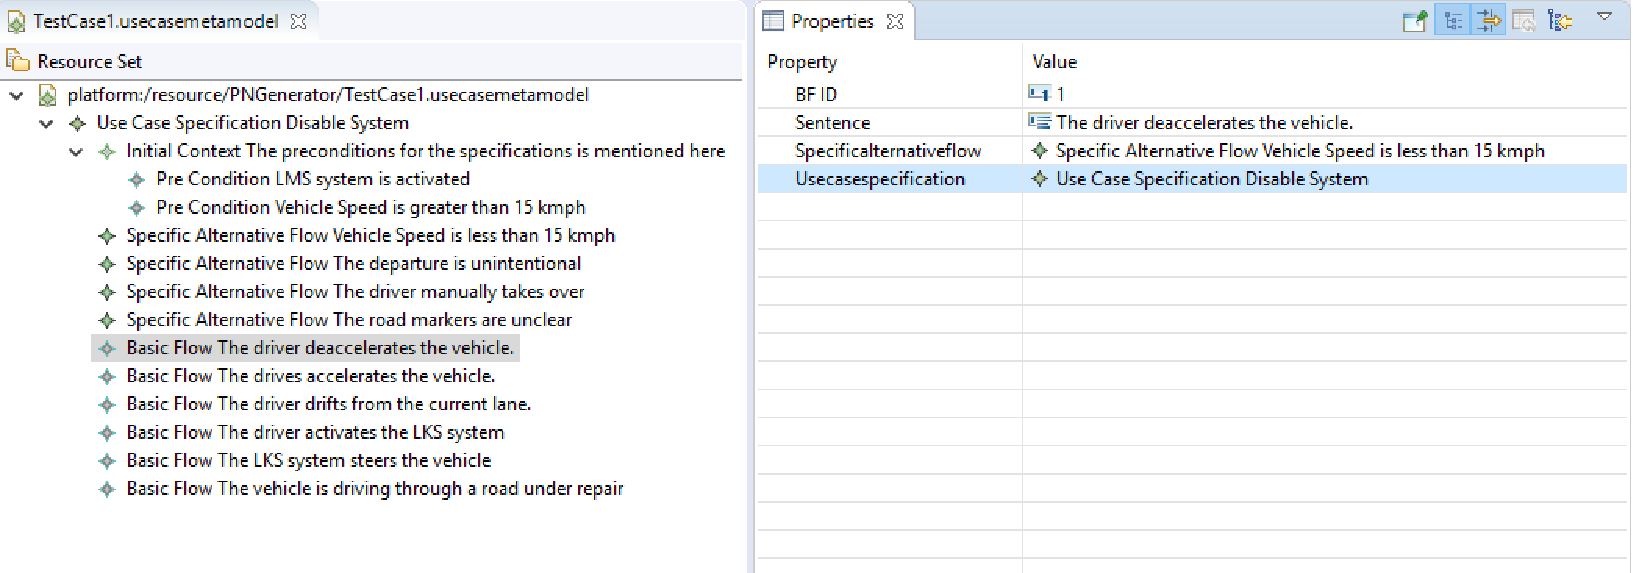
\includegraphics[width=1\textwidth]{content/images/Chapter5/Requiremens_Snip}}
\caption{Running example given as input to the tool}
\label{fig:input}
\end{figure}

\begin{figure}[htb!]
\centering
\fbox{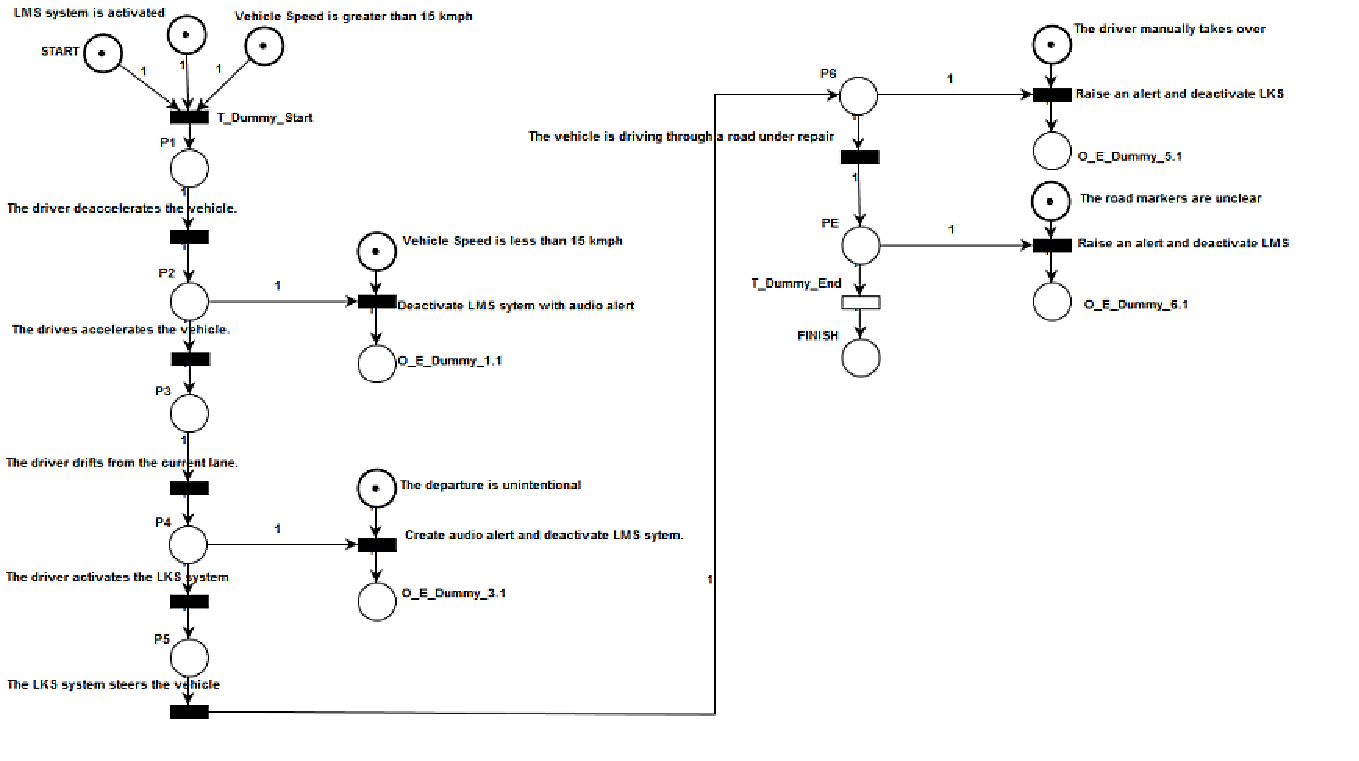
\includegraphics[width=1\textwidth]{content/images/Chapter5/FinalIntegratedPetriNet}}
\caption{Integrated Petri Net for the running example}
\label{fig:integratedpn}
\end{figure}


To give inputs to the tool, we should create an instance of the \gls{rucm} metamodel. The running example is given as input for the tool and the structure of the user input can be seen in Figure \ref{fig:input}.

\subsubsection{Model Transformations}
This section describes how the \gls{ucs} in \gls{rucm} metamodel is converted into an integrated Petri Net. Model transformations, which are the core of the MDSE technique, are used for this purpose.

The first step of the transformation process is to transform elements from \gls{rucm} metamodel to Petri Net metamodel elements. For this purpose, the concept of \gls{m2m} transformation is used and it needs specific rules for transformation from one metamodel to another.  In our tool, these rules are implemented using QVTo \cite{eclipseqvt}. 

Once this transformation is executed, we get a collection of Sub Petri Nets. These should be integrated again into a single Petri Net using the rules defined in Section \ref{integratedpngen}. These rules are again implemented using QVTo as a \gls{m2m} transformation. Appendix \ref{m2mrules} shows the implementation of these rules.

The output of the above transformation yields an integrated Petri Net. In order to make this output compatible with other Petri Net tools, the available Petri Net is converted into a standard xml file called \gls{pnml}. This transformation from Petri Net metamodel to textual representation is done using \gls{m2t} transformation implemented in Xpand language \cite{eclipsem2t}. Appendix \ref{m2trules} gives the details of this implementation. A graphical representation of the intermediate output for our running example in PIPE2 tool is shown in Figure \ref{fig:integratedpn}.

\subsection{Implementation in PIPE2 tool}
This block generates the reachability graph. The integrated Petri Net in the form of the XML file is given as input to the PIPE2 tool. From this, the reachability graph is generated using the corresponding menu in the tool. In order to use this graph in the subsequent steps, it is exported as an XML file. For this, a package is added to the existing tool and this exports the XML file in a specified template. The implementation is done using \gls{jdk}.

\subsection{Implementation in \gls{jdk} environment}
This block is responsible for the generation of test specifications and test scripts. Inputs to this section are the Reachability Graph and the \gls{pnml} file. The test specification is generated by identifying the reachable paths from the Reachability Graph and then the conditions from the \gls{pnml} file are added. For identifying all reachable paths, an \textit{All Path Search} is done from initial state to tangible states using \textit{Depth First Search Algorithm}.

\begin{figure}[htb!]
\centering
\fbox{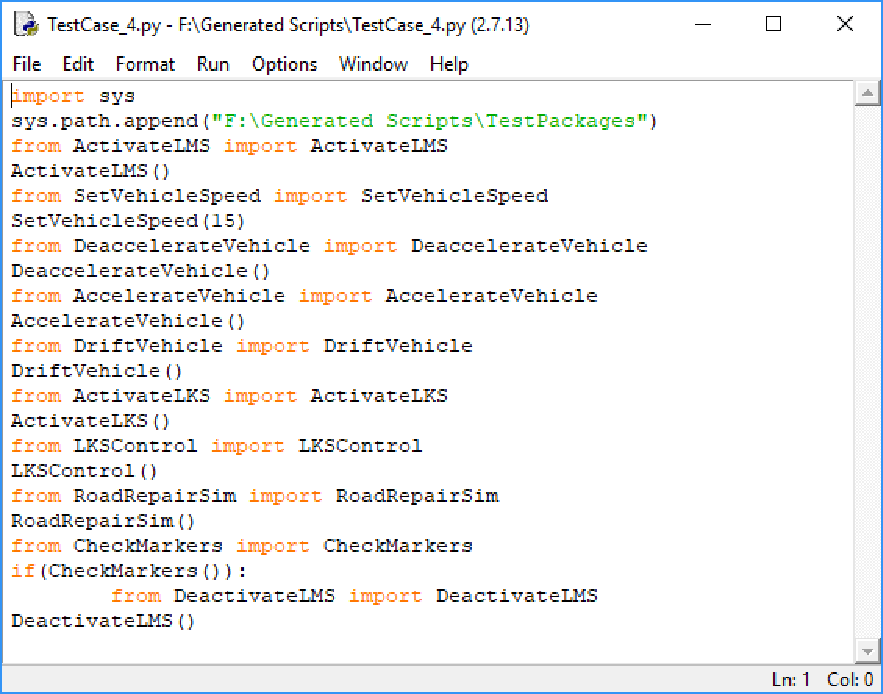
\includegraphics[width=0.8\textwidth]{content/images/Chapter5/TestScript}}
\caption{The final output of the TSTG tool}
\label{fig:testscript}
\end{figure}

Once a test specification is ready, each test case in the test specification is elicited out and the test steps for the test cases are generated using an implementation similar to a Lookup table. This Lookup table maps each test step to a package predefined in python and finally, executable test cases are generated in python. Figure \ref{fig:testscript} shows a generated test script for one of the test cases of our running example. The entire implementation is done in \gls{jdk} using Eclipse Java Standard Edition.

% !TeX spellcheck = de_DE

\chapter{Evaluation of the Tool}\label{evaluation} 
This chapter gives detailed information on how our tool is evaluated. Evaluation of the tool is done on the basis of parameters used by similar tools to access the quality of generated test scripts. These parameters facilitate correlating our tool with other tools.

The first section of the chapter speaks on the various methods and criteria used for evaluation. The second section of this chapter discusses the different results obtained from the evaluation and also compares our tool with similar tools available in the research domain.
\section{Preliminary Preparation for Evaluation}
This section gives an idea of the system to be used for evaluation, the different criteria and the procedure used for evaluation.
\subsection{System for Evaluation}
For evaluation of \gls{tsgt} tool, we use a system called \gls{lms}. The \gls{lms} is safety critical automotive software used in most of the present-day automobiles. The \glspl{srs} for \gls{lms} provided in \cite{blazysoftware} serves a foundation for our evaluation. This document provides an overview of the entire system and the various requirements needed for system development.  It also provides detailed requirements for specific functionalities and in addition includes models describing the functionality and interactions of the system. The requirements are organized in the form of use cases and there are totally 13 use cases which act as inputs for our tool.
\subsection{Evaluation Criteria}
The evaluation of the tool is based on two main criteria.
\begin{enumerate}
\item The time taken for the generation of test scripts.
\item The coverage of requirements by the generated test cases.
\end{enumerate}
\subsubsection{\textbf{Time Criteria}}

\begin{definition}
\label{def:def5}

The effort required to generate a test case is defined as the average time taken to generate the test cases \cite{elghondakly2015waterfall}.

Effort$_{TC}$   = $\displaystyle\frac{\mbox{Time taken to generate the test cases}}{\mbox{Total number of generated test cases}}$

In case of the automated process, the time taken to generate the test cases is inclusive of the time that is required to specify the requirements in \gls{rnl}, whereas in case of the manual process, it is inclusive of the time taken to convert the test cases into executable test scripts.
\end{definition}

\begin{definition}
\label{def:def6}

Test Case Productivity is defined as the ratio of the number of test steps generated to the time taken (in minutes) to generate these test steps \cite{gulechha2009software}.

Test Case Productivity (TCP)   = $\displaystyle\frac{\mbox{Number of test steps generated}}{\mbox{Total Time taken to generate the test steps}}$
\end{definition}

\subsubsection{\textbf{Coverage Criteria}}
The following criterion is necessary to analyze the quality of the test case generation process. This criterion also evaluates our methodology for Petri Net derivation since the test case generation depends upon the derived Petri Net.

\begin{definition}
\label{def:def7}

The generated test cases must ensure that all the requirements in \gls{srs} are covered at least once. This is also requirement of ISO-26262 \cite{iso201126262}, a standard for functional safety of automobiles.

Requirement Coverage = $\displaystyle\frac{\mbox{Number of requirements covered}}{\mbox{Number of requirements present in the \gls{srs}}}$  $\times 100$
\end{definition}

\begin{definition}
\label{def:def8}

The generated test cases must ensure that all possible paths from the initial place to the final place in a Petri Net are covered at least once.

Path Coverage = $\displaystyle\frac{\mbox{Number of paths covered}}{\mbox{Number of paths present}}$  $\times 100$
\end{definition}

\subsection{Evaluation Procedure}
The sequence of steps followed for evaluation of the tool is shown graphically in Figure 1. The evaluation is done by comparing the manual and automatic generation of test scripts. The \gls{srs} document provided in \cite{blazysoftware} acts as input for the domain expert. In case of manual means, the domain expert analysis the \gls{srs} document and creates the test specification. Once it is done, the tester creates the test scripts corresponding to the test specification. In case of automatic means, the domain expert writes the requirements in \gls{rnl} and provides it as an input to the \gls{tsgt} tool which directly generates the test scripts.
\section{Evaluation Results and Discussion}
This section lists out the results obtained from the evaluation process and further discusses the various inferences from the results.
\subsection{Analysis of Quantitative Data}
\subsubsection{Based on Time Criteria}
The results of the tool evaluation are first discussed with respect to time criteria discussed in Section xxxx. Table 1 and 2 describe the different parameters for manual and tool generated test scripts respectively. The tables provide data of five different use cases from our evaluation system and also the average of different parameters.

According to definition xxxx, Effort per test case is indicative of the average time required to generate each test case. The tables show that the effort required for each test case in manual method is 10.6 minutes per test case on an average whereas in automatic generation it is 1.6 minutes per test case. This denotes an 85\% improvement over the manual method.

According to definition xxxx, \gls{tcp} shows the number of test steps that can be generated in one minute. From the tables, it can be seen that our tool generated 3.3 more test steps in a minute because \gls{tcp} stands at 0.6 and 3.9 for manual and automatic methods respectively. Figure 2 shows a chart that contains the details of all the individual use cases.
From the tables it can be inferred that the total time taken for generating the test scripts manually takes 54 minutes on an average whereas the total time taken for automatic test script generation is only 13 minutes. This implies that there is a 76\% reduction in time when the tool is used for test script generation.

\subsubsection{Based on Coverage Criteria}

This segment deals with the results of the tool evaluation based on coverage criteria discussed in Section xxxx. Table 3 describes the different parameters for manual and tool generated test scripts respectively.

From the table, it can be inferred that the number of test cases generated by manual method is always less than the automatic method. The coverage percentage in case of manual method is solely dependent on the individual extracting the test cases. Hence we see difference in coverage percentage in manual method and it is arbitrary. But in the automatic method, requirement and path coverage are always 100\%. This is due to the formal method of test case generation and this also ensures that each requirement and path is covered with the generated test cases. 

\subsection{Based on Coverage Criteria}
This section compares our tool i.e. \gls{tsgt} with other closely related test script generation tools available in the research field. Figure 3 shows a graphical representation of the comparison between different approaches based on the effort per test case criterion. The data for manual and \gls{tsgt} approach are taken out from our evaluation. \cite{yue2015rtcm}provides the data for \gls{rtcm} and \gls{umtg} approach.

The pros and cons of the different approaches are discussed below. \gls{umtg} provides an exhaustive test data for test script generation but it requires domain models for test data generation. The need for domain model generation along with test data generation using \gls{ocl} increases the effort required for test case generation. \gls{rtcm} provides the best solution but it requires manual intervention to improve some of the intermediate artifacts which might increase the effort in some cases. 

The total time taken for test case generation in our tool is inclusive of the time taken to specify the \glspl{ucs} in \gls{rucm} template and to present them as input to our tool. This solely depends upon the expertise of the user in \gls{rucm} template and also the experience in our tool. The time taken for test script generation after the input section is negligible. Figure 4 shows how the total time taken for test script generation from each use case is split between different blocks in our tool. From the chart, it is obvious that the \gls{ucs} to \gls{rucm} template utilizes most of the time taken.

The advantage with our tool is that the time taken to specify complex \glspl{ucs} does not add much to the total time taken, but produces more number of test cases. This scenario can be explained with the help of a graph as shown in Figure 5. By comparing Use Case 3 and Use Case 5, there is not much difference in the time required to specify the \glspl{ucs} but there is a drastic increase in the number of test cases that are generated thereby reducing the effort required to generate them. In the manual method, it can also be seen that more complex the use cases become, lesser the number of test cases identified. The average effort required to generate a test case will improve drastically when more number of complex use cases are evaluated.

\subsection{Summary}
This section summarizes the trends observed in the evaluation results and our tool characteristics. Evaluation criteria considering time and coverability have been compared between \gls{tsgt} and manual methods. The evaluation shows that \gls{tsgt} requires 85\% less effort than the manual method and it also provides 100\% coverability. Our tool has also been compared with other similar approaches in the research field and has been found to be good. Also, the limitations of our tool in reducing the effort required for each test case has been discussed and ways to improve them are suggested. From all the above discussions, it can be concluded that that automatic test case generation using \gls{tsgt} is definitely better than manual test case generation and other existing approaches. 
%\input{...weitere Kapitel...}
\input{content/kapitel2}
\input{content/zusammenfassung_und_ausblick}
%
%
%\renewcommand{\appendixtocname}{Anhang}
%\renewcommand{\appendixname}{Anhang}
%\renewcommand{\appendixpagename}{Anhang}
\appendix
\input{content/latex-tipps}

\clearpage

%\printindex

\printbibliography

\ifdeutsch
Alle URLs wurden zuletzt am 17.\,03.\,2008 geprüft.
\else
All links were last followed on September 20, 2017.
\fi

\pagestyle{empty}
\renewcommand*{\chapterpagestyle}{empty}
\Versicherung
\end{document}
